% Options for packages loaded elsewhere
\PassOptionsToPackage{unicode}{hyperref}
\PassOptionsToPackage{hyphens}{url}
%
\documentclass[
  letterpaper,
  DIV=11,
  numbers=noendperiod]{scrartcl}

\usepackage{amsmath,amssymb}
\usepackage{setspace}
\usepackage{iftex}
\ifPDFTeX
  \usepackage[T1]{fontenc}
  \usepackage[utf8]{inputenc}
  \usepackage{textcomp} % provide euro and other symbols
\else % if luatex or xetex
  \usepackage{unicode-math}
  \defaultfontfeatures{Scale=MatchLowercase}
  \defaultfontfeatures[\rmfamily]{Ligatures=TeX,Scale=1}
\fi
\usepackage{lmodern}
\ifPDFTeX\else  
    % xetex/luatex font selection
\fi
% Use upquote if available, for straight quotes in verbatim environments
\IfFileExists{upquote.sty}{\usepackage{upquote}}{}
\IfFileExists{microtype.sty}{% use microtype if available
  \usepackage[]{microtype}
  \UseMicrotypeSet[protrusion]{basicmath} % disable protrusion for tt fonts
}{}
\makeatletter
\@ifundefined{KOMAClassName}{% if non-KOMA class
  \IfFileExists{parskip.sty}{%
    \usepackage{parskip}
  }{% else
    \setlength{\parindent}{0pt}
    \setlength{\parskip}{6pt plus 2pt minus 1pt}}
}{% if KOMA class
  \KOMAoptions{parskip=half}}
\makeatother
\usepackage{xcolor}
\setlength{\emergencystretch}{3em} % prevent overfull lines
\setcounter{secnumdepth}{5}
% Make \paragraph and \subparagraph free-standing
\ifx\paragraph\undefined\else
  \let\oldparagraph\paragraph
  \renewcommand{\paragraph}[1]{\oldparagraph{#1}\mbox{}}
\fi
\ifx\subparagraph\undefined\else
  \let\oldsubparagraph\subparagraph
  \renewcommand{\subparagraph}[1]{\oldsubparagraph{#1}\mbox{}}
\fi


\providecommand{\tightlist}{%
  \setlength{\itemsep}{0pt}\setlength{\parskip}{0pt}}\usepackage{longtable,booktabs,array}
\usepackage{calc} % for calculating minipage widths
% Correct order of tables after \paragraph or \subparagraph
\usepackage{etoolbox}
\makeatletter
\patchcmd\longtable{\par}{\if@noskipsec\mbox{}\fi\par}{}{}
\makeatother
% Allow footnotes in longtable head/foot
\IfFileExists{footnotehyper.sty}{\usepackage{footnotehyper}}{\usepackage{footnote}}
\makesavenoteenv{longtable}
\usepackage{graphicx}
\makeatletter
\def\maxwidth{\ifdim\Gin@nat@width>\linewidth\linewidth\else\Gin@nat@width\fi}
\def\maxheight{\ifdim\Gin@nat@height>\textheight\textheight\else\Gin@nat@height\fi}
\makeatother
% Scale images if necessary, so that they will not overflow the page
% margins by default, and it is still possible to overwrite the defaults
% using explicit options in \includegraphics[width, height, ...]{}
\setkeys{Gin}{width=\maxwidth,height=\maxheight,keepaspectratio}
% Set default figure placement to htbp
\makeatletter
\def\fps@figure{htbp}
\makeatother
\newlength{\cslhangindent}
\setlength{\cslhangindent}{1.5em}
\newlength{\csllabelwidth}
\setlength{\csllabelwidth}{3em}
\newlength{\cslentryspacingunit} % times entry-spacing
\setlength{\cslentryspacingunit}{\parskip}
\newenvironment{CSLReferences}[2] % #1 hanging-ident, #2 entry spacing
 {% don't indent paragraphs
  \setlength{\parindent}{0pt}
  % turn on hanging indent if param 1 is 1
  \ifodd #1
  \let\oldpar\par
  \def\par{\hangindent=\cslhangindent\oldpar}
  \fi
  % set entry spacing
  \setlength{\parskip}{#2\cslentryspacingunit}
 }%
 {}
\usepackage{calc}
\newcommand{\CSLBlock}[1]{#1\hfill\break}
\newcommand{\CSLLeftMargin}[1]{\parbox[t]{\csllabelwidth}{#1}}
\newcommand{\CSLRightInline}[1]{\parbox[t]{\linewidth - \csllabelwidth}{#1}\break}
\newcommand{\CSLIndent}[1]{\hspace{\cslhangindent}#1}

\KOMAoption{captions}{tableheading}
\usepackage[left]{lineno}
\linenumbers
\usepackage{xcolor}
\usepackage{caption}
\captionsetup[figure]{font=footnotesize}
\makeatletter
\makeatother
\makeatletter
\makeatother
\makeatletter
\@ifpackageloaded{caption}{}{\usepackage{caption}}
\AtBeginDocument{%
\ifdefined\contentsname
  \renewcommand*\contentsname{Table of contents}
\else
  \newcommand\contentsname{Table of contents}
\fi
\ifdefined\listfigurename
  \renewcommand*\listfigurename{List of Figures}
\else
  \newcommand\listfigurename{List of Figures}
\fi
\ifdefined\listtablename
  \renewcommand*\listtablename{List of Tables}
\else
  \newcommand\listtablename{List of Tables}
\fi
\ifdefined\figurename
  \renewcommand*\figurename{Figure}
\else
  \newcommand\figurename{Figure}
\fi
\ifdefined\tablename
  \renewcommand*\tablename{Table}
\else
  \newcommand\tablename{Table}
\fi
}
\@ifpackageloaded{float}{}{\usepackage{float}}
\floatstyle{ruled}
\@ifundefined{c@chapter}{\newfloat{codelisting}{h}{lop}}{\newfloat{codelisting}{h}{lop}[chapter]}
\floatname{codelisting}{Listing}
\newcommand*\listoflistings{\listof{codelisting}{List of Listings}}
\makeatother
\makeatletter
\@ifpackageloaded{caption}{}{\usepackage{caption}}
\@ifpackageloaded{subcaption}{}{\usepackage{subcaption}}
\makeatother
\makeatletter
\@ifpackageloaded{tcolorbox}{}{\usepackage[skins,breakable]{tcolorbox}}
\makeatother
\makeatletter
\@ifundefined{shadecolor}{\definecolor{shadecolor}{rgb}{.97, .97, .97}}
\makeatother
\makeatletter
\makeatother
\makeatletter
\makeatother
\ifLuaTeX
  \usepackage{selnolig}  % disable illegal ligatures
\fi
\IfFileExists{bookmark.sty}{\usepackage{bookmark}}{\usepackage{hyperref}}
\IfFileExists{xurl.sty}{\usepackage{xurl}}{} % add URL line breaks if available
\urlstyle{same} % disable monospaced font for URLs
\hypersetup{
  pdftitle={The Influence of Fluvial and Glacial Watershed Dynamics on Holocene Sediment Accumulation in Cariboo Lake, Columbia Mountains, British Columbia, Canada},
  pdfauthor={A. Cebulski \& J. Desloges},
  hidelinks,
  pdfcreator={LaTeX via pandoc}}

\title{The Influence of Fluvial and Glacial Watershed Dynamics on
Holocene Sediment Accumulation in Cariboo Lake, Columbia Mountains,
British Columbia, Canada}
\author{A. Cebulski \& J. Desloges}
\date{December 8, 2023}

\begin{document}
\maketitle
\ifdefined\Shaded\renewenvironment{Shaded}{\begin{tcolorbox}[borderline west={3pt}{0pt}{shadecolor}, boxrule=0pt, frame hidden, breakable, enhanced, interior hidden, sharp corners]}{\end{tcolorbox}}\fi

\setstretch{1.5}
\begin{center}\rule{0.5\linewidth}{0.5pt}\end{center}

A. Cebulski\textsuperscript{1,2} (ORCID ID - 0000-0001-7910-5056)

J. Desloges\textsuperscript{2} (ORCID ID - 0000-0001-8446-3034)

\textsuperscript{1}Centre for Hydrology, University of Saskatchewan,
Canada

\textsuperscript{2}Department of Geography and Department of Earth
Sciences, University of Toronto, Canada

Corresponding Author: A. Cebulski, alexcebulski@gmail.com

\begin{center}\rule{0.5\linewidth}{0.5pt}\end{center}

\pagebreak

\textbf{Abstract:} Records of sedimentation collected from Cariboo Lake,
situated in the northern Columbia Mountains, British Columbia, Canada,
are analyzed to assess Holocene fluvial and glacial watershed dynamics.
The aim of this study is to provide a proxy record of Holocene
hydroclimate and glacier change from sediment archives at a higher
temporal resolution compared to available records for the Interior
Ranges of British Columbia. Deglacial and Holocene sediment accumulation
is observed to reach a maximum thickness of 35 m in deep parts of the
lake, using sub-bottom acoustic soundings. A transition from massive to
well-layered sediments is observed in the sub-bottom acoustic record
during final phases of valley deglaciation in the region (ca. 10.5--9 ka
BP). Laminae couplets are interpreted to be deposited annually according
to two \textsuperscript{14}C dates and a varve counting chronology. Two
long cores, 2.9 and 3.8 m in length, were selected for analysis with
estimated basal dates of 2 ka BP. Trends in downcore sediment
characteristics were linked to environmental changes in the glaciated
catchment headwaters at a temporal resolution of \textasciitilde100 yrs.
Upstream lake filtering of river floodplains and lakes prevented finding
a higher temporal resolution linkage between the sediment
characteristics and headwater fluvial and glacial activity. Despite some
upstream filtering, the Cariboo River was found to be the primary source
of sediment to the long core sites. Observed grain size and varve
thickness from two long cores show above average trends which are
coincident with cooler temperatures and the primary glacier advances
over the last 2 ka.

\textbf{Keywords:} Glaciolacustrine; Varve; Hydrology; Climate; British
Columbia; Holocene

\pagebreak

\hypertarget{introduction}{%
\section{Introduction}\label{introduction}}

Climatic variability in the western Canadian Cordillera over the
Holocene contributed to several fluctuations in glacial activity with
implications for sediment accumulation in glacier-fed lakes. There is
general regional agreement between the Coast Mountains (Brown et al.,
2006; Koch et al., 2007; Menounos et al., 2004; Menounos \& Clague,
2008; Osborn et al., 2007; Ryder \& Thomson, 1986) and Canadian Rocky
Mountains (Hodder et al., 2006; Leonard, 1997; Luckman, 1988, 1993;
Luckman et al., 1993) on the timing and magnitude of the large early
Holocene retreat and late Holocene LIA advance. However, the smaller
fluctuations that occurred between these large events have less regional
agreement (Menounos et al., 2009). Furthermore, few proxy records exist
in central British Columbia, that provide a high-resolution record of
Holocene hydroclimatic variability (Gilbert \& Desloges, 2012; Hodder et
al., 2006; Maurer et al., 2012; Menounos et al., 2009). Central British
Columbia is characterized by a transitional climate between the wetter
Coast Mountain Ranges to the dryer Rocky Mountain Ranges, which may
contribute to a different response of glaciers for this region over the
Holocene.

A study by Gilbert \& Desloges (2012) of Quesnel Lake (272
km\textsuperscript{2}), 30 km south of the study area examined here,
found high rates of sediment accumulation around 10.4 ka BP during early
Holocene deglaciation, and around 8.4 ka BP sediment accumulation
declined significantly. Meaningful trends in organic matter and grain
size of Quesnel Lake sediment sequences at a sub-millennial time scale
were not detectable. Quesnel Lake is very large relative to the
contributing watershed and therefore the sediment system exhibits very
low accumulation rates and is much less sensitive to climate
variability. Within the Cariboo Lake basin, Maurer et al. (2012)
investigated the headwater On-off Lake which remained intermittently
connected to the Castle Creek Glacier on the basin divide
(Figure~\ref{fig-map-basin}). Currently the Castle Creek Glacier resides
outside of the Cariboo Lake basin, however, Maurer et al. (2012) show
that the glacier advanced north across the hydrological divide and into
the Cariboo Lake basin several times over the Holocene. Both Gilbert \&
Desloges (2012) and Maurer et al. (2012) provide a long-term but coarse
temporal resolution record of Holocene hydroclimatic variability in the
Cariboo Mountains. Additional high-resolution proxy records of Holocene
fluvial and glacial activity are needed for this transitional climate of
central British Columbia; especially for the mid to late Holocene
interval where greater regional variability in glacial responses to
climate change has been observed (Menounos et al., 2009).

Environmental proxy records that extend back beyond the modern
observable record are crucial to understanding earth system processes
(Huber \& Knutti, 2012; Nelson et al., 2016; Turney et al., 2019). Proxy
reconstructions at the sub-annual (e.g.~ice cores, tree rings, corals,
varved-sediments), to multi-decadal scales (e.g.~sediments, pollen,
boreholes) have proven useful in describing past environmental
conditions across the globe (Masson-Delmotte et al., 2013). In the case
of sedimentary sequences collected from climate sensitive glaciated
watersheds, they have been important in contributing to the regional
understanding of climate and hydrologic variability over the Holocene.
For example, researchers have utilized sedimentary sequences along with
other environmental archives to provide regional (Menounos et al., 2009)
and global (Neukom et al., 2019) reconstructions of glacier and
hydroclimatic change over the Holocene. The sensitivity and temporal
resolution of lake sediment characteristics (e.g.~varves thickness,
grain size and organic content) and their connection to regional
hydrology, temperature, precipitation patterns, and glacier extent
varies amongst glacier-fed lake studies (Desloges, 1999; Hodder et al.,
2006; Leonard, 1997; Menounos, 2006; Menounos \& Clague, 2008). Mountain
basins that exhibit a strong nival-hydrographic regime typically produce
distinct varve couplets with a fine-grained layer deposited in winter
when the lake ices over and flow velocity decreases followed by a
coarse-grained layer deposited during spring high flows (Desloges, 1999;
Hodder et al., 2007; e.g. Leonard, 1997). In contrast, lakes proximal to
the Coast Mountains of British Columbia typically show greater
variability in varve thickness due to the influence of frequent and
large fall rainstorms that produce multiple coarse laminations within a
single season (e.g. Gilbert et al., 1997; Menounos \& Clague, 2008).
Establishing a correlation between seasonal or annual trends in varve
thickness, grain size, and organic content from sediment cores to local
discharge, temperature, and precipitation is not always possible for
short time scales due to complex process interactions, watershed
connectivity and dating uncertainties (Heideman et al., 2018; Hodder et
al., 2007; Menounos \& Clague, 2008). The linkage between hydrology and
climate drivers and the lake sediment record may be limited at short
time scales (i.e.~less than 10 years) if there is a weak connectivity
between sediment production and delivery to the lake (Heideman et al.,
2018; Hodder et al., 2007; Menounos \& Clague, 2008). Trends in lake
sediment sequences are typically more representative of climate
fluctuations at longer time scales greater than 100 years as this
provides sufficient time for changes in sediment production and delivery
to propagate through the watershed (Heideman et al., 2018; Leonard \&
Reasoner, 1999; Osborn et al., 2007). Shorter timescale trends in
climate change may still be reflected in lake sediment records but with
less fidelity and confidence in the chronology.

The purpose of this research is to 1) establish an understanding of the
mechanisms that control the delivery and deposition of the fine sediment
fraction to Cariboo Lake, 2) to reconstruct the highest resolution and
longest possible sediment accumulation record from cores and acoustic
methods for this semi arid region of British Columbia, 3) determine if
the sediment accumulation record contains a signal from fluvial and
glacial activity driven by regional to continental hydroclimate change,
and 4) ascertain how this record of hydroclimatic variability differs
from other records collected in the Coastal and Rocky Mountains.

\hypertarget{materials-and-methods}{%
\section{Materials and methods}\label{materials-and-methods}}

\hypertarget{study-area}{%
\subsection{Study Area}\label{study-area}}

Cariboo Lake is located in the northern foothills of the Columbia
Mountains, 85 km northeast of Williams Lake, British Columbia
(Figure~\ref{fig-map-basin}). The lake is separated into two basins by a
large alluvial fan building cross-valley from Keithley Creek
(Figure~\ref{fig-map-lake}). The main Cariboo Lake basin, to the
northeast of Keithley Creek, receives discharge from an area of 2636
km\textsuperscript{2}, which is filtered by three upper watershed lakes:
Issac Lake, Lanezi Lake, and Ghost Lake (Figure~\ref{fig-map-basin}).
While these lakes are more proximal to glacial activity, and may contain
sediment archives that are more closely linked to headwater changes in
fluvial and glacial activity, higher sediment accumulation rates
expected for these lakes, and their remote location, would have made it
very difficult to retrieve a long-term sediment record. With this
upstream filtering, Cariboo Lake has a lower sediment accumulation rate
which presented a more accessible option to retrieve a sediment record
that spans a longer time interval.

The watershed relief ranges from 2600 m in the eastern Cariboo Mountain
headwaters to 600 m at the western Cariboo Lake outlet. The lake area to
watershed area ratio of the main Cariboo Lake basin is 0.3\%. The
southwest to northeast, 75 km long watershed spans a precipitation
gradient ranging from 1370 mm yr\textsuperscript{-1} in the headwaters
to 477 mm yr\textsuperscript{-1} at the semi-arid outlet to the lake.
The Cariboo Lake watershed has 75 km\textsuperscript{2} of permanent ice
cover which covers 3\% of the total watershed (Bolch, 2008). The most
extensive glaciated terrain is proximal to Mt. Lunn roughly 60 km
upstream of Cariboo Lake (Figure~\ref{fig-map-basin}). The Cariboo Lake
basin hydrology is inferred from the Water Survey of Canada station
08KH003 (Albers, 2017) 20 km downvalley from the Cariboo Lake outlet
(Figure~\ref{fig-map-basin}). The watershed is snow- and glacier-melt
dominated with average 1971-2000 monthly runoff peaking in June (220 mm)
and low-flows that occur between December and March (15--25 mm)
(Figure~\ref{fig-cl-hydro}, A). From December to March air temperature
is mostly below 0 °C and precipitation falls primarily as snow
(Figure~\ref{fig-cl-hydro}). The bathymetry of the lake reaches a
maximum depth of just over 50 m in two deep holes within the central
part of the main Lake basin (Figure~\ref{fig-map-lake}). These deep
holes provide some evidence of pre-Holocene glacial scouring, suggesting
that the extent of ice may have reached the lakes current position.

Upper watershed Lanezi Lake and Sandy Lake contrast significantly in
maximum depths at 170 m and 6 m, respectively
(Figure~\ref{fig-map-basin}). The Matthews River, which meets the
Cariboo River below Lanezi Lake, is filtered by Ghost Lake and provides
an important connection to meltwater sources draining several alpine
glaciers including the largest area of ice (10 km\textsuperscript{2}) in
the Cariboo Lake watershed, proximal to Roberts Peak
(Figure~\ref{fig-map-basin}).

\hypertarget{field-methods}{%
\subsection{Field Methods}\label{field-methods}}

A field campaign was conducted during the summer of 2017 to collect
sub-bottom acoustic soundings, dredge samples, and sediment cores.
Thirty-four kilometres of sub-bottom acoustic soundings were collected
across Cariboo Lake using a 10 kHz StrataBox 3510 HD
(Figure~\ref{fig-map-lake}). An Ekman dredge was used to collect 20
samples from the lake bottom, following a longitudinal transect down
Cariboo Lake, each yielding \textasciitilde730 cm\textsuperscript{3} of
surficial sediment (Figure~\ref{fig-map-lake}). The dredge samples were
sub-sampled in the field using an 8 cm diameter PVC cylinder. This
resulted in 20 short cores each containing about 450
cm\textsuperscript{3} of sediment. Sub-sampling the dredge samples
allowed for better preservation of the sediment stratigraphy compared to
short cores taken directly in the lake. The Ekman dredge cores ranged
from 6--12 cm in length. The sediment not captured in the PVC cylinder
was kept as a bulk sediment sample.

Four long sediment cores (V1--V4) were collected using a Rossfelder
submersible vibracorer with a 6 m long, 6 cm diameter, aluminum pipe
(Figure~\ref{fig-map-lake}). Sediment cores V1--V4 were retrieved at
deep mid-lake locations to ensure the cores consisted of a higher
fraction of fine clastic sediments. It was anticipated that the
transport of coarser-grained sediments from non-glaciated tributaries
would be limited to areas proximal to the lake's perimeter. Some
contribution of organic matter and clastic sediments to the long-cores
from the smaller sidewall tributaries is anticipated. The extent of this
contribution is assessed using the Ekman surficial cores. Cores V1 and
V2 in the main Cariboo River basin were selected for detailed analysis
as these two cores had the highest fraction of fine clastic sediments,
their sediment stratigraphy was well preserved, and they both had
organic material for \textsuperscript{14}C dating. Cores V3 and V4 taken
closer to the Frank Creek and Keithley Creek deltas also had higher
fractions of coarse grained sediments and core disturbance and were not
analyzed in detail.

\hypertarget{laboratory-methods}{%
\subsection{Laboratory Methods}\label{laboratory-methods}}

Long and short cores were split longitudinally with one half preserved
as an archive and the other as a working half. The working half samples
were prepared for imaging by scraping the core parallel to the sediment
laminae to create a flat surface which showed the sediment stratigraphy.
The short and long sediment cores were analyzed for laminae thickness,
organic content, and particle size. The working halves of long cores V1
and V2 were subsampled with 2 cm\textsuperscript{3} of sediment
extracted at a 5 cm interval, with additional samples taken within
stratigraphic facies that had visual changes in grain size and
lamination patterns. Laminae couplets observed on the working halves
were digitally counted and measured for thickness using the ImageJ
software (Schneider et al., 2012). Uncertainty in laminae counting is
attributed to sections of core with indiscernible laminae formation,
undercounting, and subjectivity in classifying the occasionally thicker
(4--47 mm thick) graded to massive laminae/beds. The uncertainty of the
laminae counting in this study was inferred from Ekman short cores (E12,
E13, E14) which had statistically similar sediment accumulation rates.
The varve counting error was estimated by counting the number of
couplets down to a depth of 5 cm in each Ekman core. The top section of
cores V1 and V2 were disturbed during coring which prevented counting
and measurement of laminae couplets in 11 cm of V1 and 7 cm of V2. The
absence of clear marker laminae and limited overlap between the long
cores and short cores prevented anchoring of the long cores to the short
cores.

Organic matter was approximated from percent weight loss-on-ignition
analysis (550 °C) (Smith, 2003; Walter E. Dean, 1974). Grain size
analysis was conducted using a Mastersizer Particle Size Analyzer 3000.
Samples were prepared following methods by Gray et al. (2010) to remove
organic material. Three sequential aliquots of 20\%
H\textsubscript{2}0\textsubscript{2} were added until the sample stopped
reacting. To prevent flocculation of sediment grains the samples were
dispersed in 0.05\% solution of sodium hexametaphosphate for 24 hours.
Grain size was measured three times for each sample, resulting in an
average standard deviation of ± 0.01 µm.

The chronology of both long cores was reconstructed from Accelerator
Mass Spectrometry (AMS) \textsuperscript{14}C ages of organic material
(twigs and a conifer needle) found within the cores, and a chronology
derived from laminae couplet counting on working core images. The
\textsuperscript{14}C calibration was performed using Bchron, a Bayesian
statistical age-model software package for R (Haslett \& Parnell, 2008;
Parnell et al., 2008; Parnell et al., 2011) and the IntCal20 calibration
curve (Reimer, 2020). All data analysis and figure production were
produced using the R language (R Core Team, 2022).

\hypertarget{results}{%
\section{Results}\label{results}}

\hypertarget{sub-bottom-acoustics}{%
\subsection{Sub-bottom Acoustics}\label{sub-bottom-acoustics}}

Acoustic stratigraphy from six Transects (Figure~\ref{fig-map-lake})
reveal the range of morphologies and character of infilling sedimentary
deposits in Cariboo Lake (Figure~\ref{fig-acoustics}). Acoustic
penetration is limited in Transects A and E by coarse sediments proximal
to river fan-deltas across Cariboo Lake (see triangle symbols in
Figure~\ref{fig-map-lake} for fan-delta locations). Acoustic signal
penetration, resolution and distinctive acoustic layering improves
significantly along the thalweg of the lake bottom away from the main
Cariboo River delta along Transects B, C, and D. In the Frank Creek and
Keithley Creek sub-basins acoustic penetration is reduced along Transect
E and F, respectively. The diagonal lines across all panels
(cross-hatching) in Figure~\ref{fig-acoustics} is observed over most of
the acoustic record due to errant electrical interference from the
research vessel that could not be resolved. However, the interference
does not affect the overall quality of the acoustic results in the six
Transects (Figure~\ref{fig-acoustics}).

Transect B, 3.5 km from the Cariboo River delta, has acoustic reflectors
with 1--2 m separation that lie conformably over a hummocky basement
(Figure~\ref{fig-acoustics}, B - i). The acoustic basement drops off
below the observable record near the south channel-like depression.
Well-structured layering extends across the south side of the Transect
but pinches out towards the north shore (Figure~\ref{fig-acoustics}). On
the south side of Transect B, the thickness of acoustically
well-stratified deposits ranges from 10--20 m.

Acoustic penetration in the acoustic record increases 4.5 km from the
Cariboo River delta along Transect C, where the maximum sediment
thicknesses of 35 m are observed (Figure~\ref{fig-acoustics}, C). The
acoustic basement is interpreted to be either bedrock or coarse-grained
glacial sediment from the Last Glacial Maximum
(Figure~\ref{fig-acoustics}, C -- i). Two sediment facies are observed
above the acoustic basement based on geometry and the strength and
continuity of reflectors. The lower unit, facies A, has a thickness of
\textasciitilde12 m along undisturbed sections
(Figure~\ref{fig-acoustics}, C - A) and is more massive to weakly
acoustically layered. Two sharp-crested v-shaped notches in the middle
of Transect C are interpreted as unconformities
(Figure~\ref{fig-acoustics}, C). The channels are the same as those in
Transect B (Figure~\ref{fig-acoustics}, B) and are interpreted to be
scour channels formed by erosive, higher energy, turbidity currents that
likely date to deglaciation of the lake basin. Facies A is comprised of
a lighter grey tone representing coarse-grained sediment and lacks
parallel reflectors indicating a higher energy and more rapid deposition
of coarser lacustrine sediment. Facies B begins with high-amplitude
parallel reflectors with 2--3 m separation and conforms well with facies
A below (Figure~\ref{fig-acoustics}, C). Facies B has an average
thickness of \textasciitilde10 m and reaches a maximum thickness of 13 m
where it infills two scour channels (Figure~\ref{fig-acoustics}, C - ii
\& iii).

Transect D, to the northeast of the Frank Creek delta has well-layered
sediments in the top 5--10 m and transitions to poor acoustic
penetration below this (Figure~\ref{fig-acoustics}, D). The parallel
reflectors observed in the uppermost sediment layers of Transect D have
a thickness of 2--3 m and have a higher amplitude compared to facies B
in Transect C. Some slumping of sidewall sediments is observed on the
south sidewall (Figure~\ref{fig-acoustics}, D).

\hypertarget{spatial}{%
\subsection{Spatial Trends in Surficial Sediment}\label{spatial}}

The surficial sediment cores show declining trends in grain size and
laminae thickness with distance from the main Cariboo River delta.
Trends in percent organic matter (OM) of surficial sediment cores were
not found to exhibit systematic patterns with distance down-lake
(Figure~\ref{fig-ekmanSeds}, C). The steep decline in grain size
suggests that larger sand-sized sediments (63--2000 µm) are sensitive to
distance from fan deltas, while smaller silt-sized (2--63 µm) and
clay-sized (0.01--2 µm) sediments are transported further down-lake. The
highest percent of silt (86.5--89.6\%) and clay (9.3--14.4\%) sized
sediments are observed between 3 and 6.5 km from the Cariboo River
delta, proximal to the long core sampling locations. Higher
D\textsubscript{50} grain size and percentage of sand sized grains were
also found proximal to the Frank Creek fan-delta and within the Keithley
Creek sub-basin (Figure~\ref{fig-ekmanSeds}, A \& B).

Proximal to the Cariboo River delta the structure of the surficial
sediments exhibits massive layering, erosive contacts and the fraction
of sand grains greater than 60\%. A sand-bed with a thickness of 1 cm
was observed in E1, the core closest to the Cariboo River delta
(Figure~\ref{fig-ekmanImgs}, A). In the main Cariboo River basin, core
E13, retrieved 5.24 km from the Cariboo River delta and from a depth of
40 m, contained fine, rhythmically laminated sediment
(Figure~\ref{fig-ekmanImgs}, B).

Sediment cores E9--E15 and E18--E20, retrieved from areas distal to the
main Cariboo River delta, at lake depths of 30--50 m, have a high
fraction of silt and clay sediment and exhibit a rhythmic sequence of
fine-grained dark layers overlain by coarse-grained light layers
(Figure~\ref{fig-ekmanImgs}, B \& C). The sediment stratigraphy observed
within cores E9--E15 and E18--E20 are similar to annual laminations
(varves), which occur in lakes that have sufficient seasonal variation
in river and sediment discharge as well as lake stratification (Cockburn
\& Lamoureux, 2008; Desloges, 1999; Heideman et al., 2015; Hodder et
al., 2006; Zolitschka et al., 2015). In the Cariboo Lake basin, winter
low flows, lake-ice cover, and lake stratification reduce the velocity
of lake currents and contribute to the deposition of fine-grained
sediments on the lake bottom. During spring snowmelt high flows,
coarser-grained sediments are deposited from higher energy lake
currents. Additional deposition of coarse-grained sediment may also
result from abnormally high discharge events caused by large rainfall
events, rain-on-snow events, rapid melt of glaciers and snowpack during
heat waves, and/or turbidity currents due to delta collapse (Sabatier et
al., 2022). Coastal lakes in western Canada that are frequented by large
rainstorms and mid-winter melt events exhibit multiple laminae couplets
deposited in a given year (Menounos \& Clague, 2008). However, the
distinct spring snowmelt-dominant hydrological regime of the Cariboo
Lake watershed suggests the deposit of multiple coarse-grained laminae
in a single year is rare (Figure~\ref{fig-cl-hydro}). Coarse-grained
deposits are still possible in Cariboo Lake due to turbidity currents
from delta slumping/foreset failures, however turbidites were only
observed in Ekman cores proximal to river deltas (e.g.
Figure~\ref{fig-ekmanImgs}, A). While the sediment stratigraphy of Ekman
cores E9--E15 and E18--E20 resemble varves, further analysis of the
Cariboo Lake long-cores and \textsuperscript{14}C chronology are used to
confirm this.

\hypertarget{sediment-accumulation-chronology}{%
\subsection{Sediment Accumulation
Chronology}\label{sediment-accumulation-chronology}}

\hypertarget{chronology}{%
\subsubsection{Chronology}\label{chronology}}

Organic material for \textsuperscript{14}C dating in the clastic
dominated cores was extremely limited. A search for tephra was made
through careful magnified inspection of visual colour changes. None were
found using this method. Westgate (1977), Hallett et al. (1997) and
Maurer et al. (2012) indicate that this area of British Columbia has had
episodic volcanic ash inputs from significant eruptions that predate
2100 cal BP but nothing since. AMS \textsuperscript{14}C dates obtained
for cores V1 and V2 are presented in Table~\ref{tbl-amsDates} and
provide limited temporal control and evidence of sediment accumulation
rates for the long cores. A small twig from V1 at 343 cm and a conifer
needle and twig which were combined into one sample at V2, with an
average depth of 281 cm, yielded ages 1743--1884 cal BP and 1874--2044
cal BP, respectively. Figure~\ref{fig-amsRates} shows the
\textsuperscript{14}C chronology for V1 and V2 compared to the laminae
couplet chronologies for V1, and V2. The \textsuperscript{14}C dates
from samples V1 and V2 yield accumulation rates of 1.81 ± 0.07 mm
yr\textsuperscript{-1} and 1.37 ± 0.05 mm yr\textsuperscript{-1}
respectively.

Ekman surficial core 13 (E13) is most proximal to the V2 long core
(Figure~\ref{fig-map-lake}) and exhibits similar sediment accumulation
compared to the V1 and V2 \textsuperscript{14}C chronology and laminae
chronology of V2 (Figure~\ref{fig-amsRates}, inset). If one couplet
corresponds to one year of sedimentation, then the resulting sediment
accumulation rate would be 1.98 ± 0.19 mm yr\textsuperscript{-1}, which
is consistent with those computed from the \textsuperscript{14}C
chronologies of V1 and V2 (Figure~\ref{fig-amsRates}). The light-dark
couplets shown in Figure~\ref{fig-ekmanImgs}, are similar to annual
deposits noted in dozens of other varved lakes throughout BC (e.g.,
Hodder et al., 2006). Therefore, the couplets within the Ekman cores are
interpreted as varves. Higher accumulation rates are expected for the
Ekman samples as they are not subjected to the same level of compaction
as deeper sediment in the long cores.

By comparison with nearby lakes, accumulation rates in areas proximal to
river inputs in Quesnel Lake were measured to be about 0.72 mm
yr\textsuperscript{-1} (Gilbert \& Desloges, 2012). Sediment inputs are
expected to be lower in the much larger Quesnel Lake compared to Cariboo
Lake, with more arid and less glaciated portions of the Quesnel Lake
watershed contributing to that lower rate. The AMS accumulation rates of
1.81 ± 0.07 mm yr\textsuperscript{-1} and 1.37 ± 0.05 mm
yr\textsuperscript{-1} in Cariboo Lake are as expected for a smaller
watershed with a higher fraction of glacier cover compared to Quesnel
Lake (Hodder et al., 2006). The \textsuperscript{14}C dates from samples
V1 and V2 provide an important control when interpreting the inferred
temporal pattern of sediment inputs to Cariboo Lake.

Three distinct sediment facies were observed in both V1 and V2:
discernible couplets, indiscernible couplets (disturbed facies) and
graded turbidites. The similarity in couplet structure and thickness
between cores V1 and V2 and processes that deliver sediment into Cariboo
Lake strongly suggested these are varves. This interpretation is also
supported by the two \textsuperscript{14}C dated samples from cores V1
and V2 which corresponded reasonably well with the couplet count
chronology at the same depth (Figure~\ref{fig-amsRates}). The slightly
lower sediment accumulation rate at V2 is interpreted to be due to its
location 3 km further down lake. Differences between the
\textsuperscript{14}C and varve chronologies for each core were
attributed to uncertainties with couplet counting and AMS
\textsuperscript{14}C dating.

The uncertainty of the laminae counting method is inferred from Ekman
surface cores by counting laminae down to a common specified depth of 5
cm for three Ekman cores E12, E13, E14 which are proximal to V1 and V2
(Figure~\ref{fig-map-lake}). The Ekman laminae counting analysis
resulted in an uncertainty estimate of the counting method of about 10\%
or 1 miscounted varve per 10 years. This counting error of 10\% is
higher than the varve counting error of 0.7\% in Menounos \& Clague
(2008) and 0.7--6\% in Zolitschka (1991). The dominant spring melt of
this basin suggests multiple high flow events are rare
(Figure~\ref{fig-cl-hydro}). This hypothesis is also supported by
Figure~\ref{fig-amsRates} which shows a negative bias of the varve
chronology compared to the calibrated \textsuperscript{14}C age-depth
model.

Instantaneously deposited (event-based) turbidites were identified if
laminae/beds had D\textsubscript{50} grain size greater than 3 standard
deviations from the mean and/or thickness greater than 6 standard
deviations for V1 and 2 standard deviations for V2 from the mean.
Figure~\ref{fig-varve-turb} examples show the difference in regular
laminae compared to an event-based turbidite bed. Turbidite beds
observed in V1 and V2 were well defined and graded fining upward
(Figure~\ref{fig-varve-turb}, d). These turbidite beds are similar in
structure to those described in Sabatier et al. (2022) as originating
from a flood, glacial lake outburst flood, or delta collapse event.
Since the Cariboo River upstream of Cariboo Lake is filtered by
headwater proglacial lakes, it is likely the coarse sediment grains
observed within the turbidite beds at the distal V1 and V2 sites are
from localized sidewall tributary floods. Collapse of the foreslope of
an oversteepened Cariboo delta is also possible.

Where possible the thickness, grain size statistics, and percent organic
matter (OM) were analyzed for each event layer. The increased grain size
and greater thickness of the turbidites illustrate the high sediment
flux during these events compared to the annual couplets
(Table~\ref{tbl-turbTbl}). The composition of sediment grains within the
event-based layers were all characterized by a coarser single mode with
less than 0.01\% clay, over 98\% silt and less than 1\% sand. The grain
size distribution for the annual couplet sediments is characterized by a
bi-modal distribution with an average composition of 16\% clay, 83\%
silt, and less than 1\% sand. Figure~\ref{fig-amsRates} shows that most
event-based layers observed within V1 and V2 occurred at similar times.
Since each of the event-based layers contain sediment deposited over a
single, potentially localized event, they were removed from the
varve-based chronology and trend analyses of varve thickness, grain
size, and percent organics.

The varve-based chronology is based on the counting of discernible
couplets with the instantaneously deposited turbidite facies removed.
Indiscernible couplets in the disturbed-massive units makes interpreting
the time elapsed over each of these units difficult
(Figure~\ref{fig-varve-turb}, C). To compensate for the depth intervals
associated with the disturbed sections, a 30-year moving average of
sediment accumulation rates from immediately above and below the
disturbed sections were used to interpolate accumulation rates over each
facies (see method described in Menounos \& Clague, 2008). For core V1,
couplets were counted down to a core depth of 343 cm, where the organic
material for \textsuperscript{14}C dating was retrieved. This resulted
in a couplet-derived age estimated of 1419 ± 142 yr BP compared to the
two-sigma calibrated \textsuperscript{14}C age range of 1820-1918 cal
BP. For core V2, the couplets yielded an age of 1792 ± 180 yr BP for the
organic material at a depth of 281 cm, . The better alignment between
the couplet counting age and the AMS derived age in V2 can be attributed
to the higher degree of core disturbance in V1 compared to V2. Sections
that had indiscernible couplets may have resulted in some undercounting
within core V1. While there is substantial uncertainty in both the varve
counting and AMS \textsuperscript{14}C dating methods, the overlap in
the uncertainty bounds in Figure~\ref{fig-amsRates} for V2, similar
timing of turbidite events and general agreement between the two
chronologies for V1 suggests the laminae couples may be deposited
annually. Additional \textsuperscript{14}C analysis is required to
conclusively determine the couplets are varves, however the majority of
evidence presented here suggests this is the case.

The basal age for each core is estimated using both the varve counting
method and a linear extrapolation of the \textsuperscript{14}C
chronology. The basal age of V1 at 378 cm is approximately 1537 ± 154
varve yr BP based on the varve chronology and the two-sigma calibrated
\textsuperscript{14}C range is 1931--2086 cal BP. The basal age of V2 at
282 cm is about 1797 ± 180 varve yr BP based on the varve chronology and
the two-sigma calibrated \textsuperscript{14}C range is 1902--2051 cal
BP. The closer alignment of the \textsuperscript{14}C and varve
chronology at V2 gives greater confidence in the V2 age model used for
reconstructing the timing of Holocene sedimentation patterns for this
core. Since V1 has a greater spread between the two chronologies, there
is less confidence in the chronology of this core. However, given the
physical mechanisms that control sedimentation in Cariboo Lake it is
likely both cores primarily contain couplets that are deposited
annually.

\hypertarget{sediment-laminae-statistics}{%
\subsubsection{Sediment Laminae
Statistics}\label{sediment-laminae-statistics}}

A time series of varve thickness (as standardized departures) is
presented in Figure~\ref{fig-varves-a}, using only discernible couplets.
Event-based turbidites have been removed and indiscernible facies are
represented as gaps. The chronology for this time series was derived
using a linear interpolation from the median calibrated
\textsuperscript{14}C date of each core (Table~\ref{tbl-amsDates}). The
mean varve thickness for V1 is 2.4 mm and for V2 is 1.5 mm. The time
series of varve thickness measured from V1 and V2 illustrates trends in
suspended sediment delivery to Cariboo Lake (Figure~\ref{fig-varves-a}).
The 30-year average varve thickness are largely above average from
0--750 CE, for both V1 and V2, with a stronger signal observed for V1
which is closer to the main Cariboo River outlet. Below average varve
thickness is observed at both V1 and V2 from 750--1600 CE. After 1600
CE, trends in varve thickness between the two cores depart, with V2
above average during the Little Ice Age and V1 remains below average.
Sub-centennial trends are not reported due to the coarse temporal
control for both V1 and V2.

\hypertarget{grain-size}{%
\paragraph{Grain Size}\label{grain-size}}

The mean D\textsubscript{50} grain size is 7.6 ± 0.01 µm at V1, which is
closer to the Cariboo River delta, compared to 6.3 ± 0.01 µm at V2. The
temporal pattern in standardized departures of D\textsubscript{50} grain
size between the two cores shows a consistent pattern
(Figure~\ref{fig-particle}). Both V1 and V2 have above average grain
size between 0--700 CE and below average from 700--1500 CE. After 1500
CE, grain size follows an increasing trend with average to above average
grain size. V1 shows an earlier increase in grain size compared to V2.
While couplet thickness does not increase substantially over the LIA
interval, gain size does. Overall, grain size fluctuations at a temporal
resolution of about 100-years shows good correspondence between the two
cores over the last 2000 years.

\hypertarget{organic-matter}{%
\paragraph{Organic Matter}\label{organic-matter}}

The average percent organic matter (OM) of V1 and V2 is similar at
4.76\% and 4.80\%, respectively, suggesting that the flux of
allochthonous organic material to the core locations is not dependent on
distance from the main Cariboo River as it is easily transported through
the lake due to low density. This is also supported by OM measured
within the Ekman bulk samples, where a systematic down-lake relationship
was not observed (Figure~\ref{fig-ekmanSeds}, C). Figure~\ref{fig-loi}
shows the percent OM for both V1 and V2. Higher levels of organic
content are shown in V1 and V2 from 0--1000 CE and mostly below average
from 1000--2000 CE. Specific periods of above average OM for V1 occur
around CE 50--500, 650--1150, around 1300 and 1750--1850. OM in V2
matches above average values in the interval CE 250--550 and 650--950.

\hypertarget{discussion}{%
\section{Discussion}\label{discussion}}

Cariboo Lake was selected to test the utility of sediment archives from
moderate sized glacier-fed lakes as a proxy of catchment-wide fluvial
and glacial activity. The results from acoustic soundings and short-core
sediment characteristics supports the hypothesis that sediment delivered
from the Cariboo River is the primary source of sediment to Cariboo
Lake. Rhythmically laminated silt and clay transported primarily through
suspended sediment processes from the Cariboo River were observed in the
deep basins of the lake, which lie distal to river deltas where
turbidity currents and bedload transport processes are reduced. Although
coarser grained sediments from discrete turbidite flows were observed
proximal to sidewall tributary deltas (Figure~\ref{fig-ekmanSeds}), they
are only transferred to deep lake deposits during rare episodic events
(Table~\ref{tbl-turbTbl}). The long core (V1 and V2) sediment is
composed of nearly 99\% silt and clay resulting in laminae couplets that
are inferred to have been delivered via suspended sediment from the
Cariboo River. After removal of instantaneous turbidites, the long core
sediment records are thought to be most representative of trends in
Cariboo River discharge influenced by temperature and precipitation
rather than isolated events and inputs from nearby tributaries and
hillslopes.

Evidence of late Pleistocene deglaciation in the Cariboo Lake region is
provided by sub-bottom acoustic results. A maximum deglacial sediment
thickness of \textasciitilde35 m puts Cariboo Lake in the middle to
lower range of Holocene sediment inputs in Canadian Cordilleran lakes
(Gilbert \& Desloges, 2012). The study of smaller Mud Lake, in the Rocky
Mountains to the east of Cariboo Lake (Figure~\ref{fig-map-basin},
inset) was evaluated by Hodder et al. (2006), who found the early phases
of deglaciation and lake sediment infill started just prior to 9.6 ka
BP. Gilbert \& Desloges (2012) indicate deglaciation of the north and
west arms of nearby Quesnel Lake was likely complete by 8.6 ka BP.
Menounos et al. (2017) describe substantial loss of the Cordilleran Ice
Sheet across western Canada as early as 14.0 ka BP. The Cariboo Lake
acoustic results contribute to this regional record however the inferred
bottom dates present uncertainty in the actual timing.

Unlike many other deglacial sediment packages in Canadian Cordilleran
lakes, the sediment infill in Cariboo Lake has been subject to deep
trenching during deglaciation and the early Holocene
(Figure~\ref{fig-acoustics}, C). The troughs, with sediment infills
occurring at different times, suggest the presence of highly erosive but
intermittent bottom currents during deglaciation and possibly into the
earliest Holocene. Energetic flow of cold sediment-rich meltwater flow
would be required, suggesting proximity of an actively retreating valley
glacier. The absence of lower elevations moraines in the valley upstream
of Cariboo Lake might indicate rapidly retreating ice into headwater
locations. However, in general, moraines indicative of stagnant ice
fronts in lower elevation settings are not common elsewhere throughout
much of the eastern Cordillera, suggesting that valley glacier
development was limited (Menounos et al., 2017).

In contemporary ice-proximal lakes with extensive coverage of active
glaciers, high accumulation rates have been observed to be between 0.5 m
yr\textsuperscript{-1} (Crookshanks \& Gilbert, 2008) and as high as 1 m
yr\textsuperscript{-1} (Gilbert et al., 1997) during deglaciation.
Similar high accumulation rates in the late-glacial are inferred to have
occurred in Quesnel Lake (Gilbert \& Desloges, 2012), resulting in a
thick pre-Holocene sediment package. Evidence for high deglacial
sediment accumulation rates in Quesnel Lake, resulting from large,
dynamic glaciers, suggests that similar basins such as Cariboo Lake also
experienced high accumulation rates during deglaciation.

Two Transects of sub-bottom acoustic records analyzed within Cariboo
Lake provide evidence of high sediment accumulation rates during the
early Holocene. Sub-bottom acoustic records from Transect B, which is
proximal to the V1 core, indicate an upward transition from
massive-unlayered (Facies A) to well-stratified deposits (Facies B) at
about 20 m below the lake floor (Figure~\ref{fig-acoustics}). Assuming a
maximum Holocene sediment accumulation rate of approximately 1.9 mm
yr\textsuperscript{-1} from V1, this would put this transition at about
10.5 ka BP. Transect C, located in between cores V1 and V2, shows the
transition of Facies A to B occurring at a depth of around 15 m
(Figure~\ref{fig-acoustics}). Using a combined V1 and V2 average
Holocene sediment accumulation rate of 1.7 mm yr\textsuperscript{-1} in
this region of the lake, puts the transition from Facies A to B at
around 9 ka BP for Transect C, slightly later than the Transect B
estimate. The massive structure of Facies A is inferred to be due to
high rates of sediment delivery as glaciers retreated upvalley during
the early Holocene after the formation of the deep trenches. The
well-layered sediment of Facies B, along with the continuation of
laminae couplets observed in cores V1 and V2 over the last 2 ka,
suggests that glaciers reduced in extent at the start of the Holocene
but did not disappear completely.

During the early Holocene sediment accumulation rates are generally
lower across western Canada due to reduced glacier extent and warm
temperatures (Koch et al., 2007; Luckman, 1988, 1993; Menounos et al.,
2004; Osborn et al., 2007). Therefore, the estimated basal ages of
Facies A and B may be much older if the actual accumulation rates were
lower at that time. The timing of the transition between these two
facies is similar to the onset of deglaciation and start of the Holocene
sediment package within Mud Lake, BC (Hodder et al., 2006) around 9.6 ka
BP, at Moose Lake, BC (Desloges, 1999) around 10.3 ka BP, at Quesnel
Lake, BC (Gilbert \& Desloges, 2012) around 8.6 ka BP, and at the Upper
Bow River, AB (Leonard \& Reasoner, 1999) around 11.7 ka BP. Warming in
the early Holocene around 9.10--6.70 ka BP in the Canadian Rockies
specifically (Luckman, 1986), and British Columbia more generally
(Clague et al., 1989; Steinman et al., 2019), led to two possible
sedimentation regimes. The first is characterized by more regular
seasonality of sediment inputs and laminae couplet formation due to the
influence of glaciers that persisted in the Canadian Rockies through the
warm interval (e.g.~Mud Lake, Hodder et al., 2006). The second is
characterized by much lower sediment accumulation and seasonality
resulting from the widespread disappearance of glaciers during the warm
interval (e.g.~Moose Lake, Desloges, 1999). Sub-bottom acoustic records
from Cariboo Lake show continuous sediment accumulation rates throughout
the Holocene. Gilbert \& Desloges (2012) also observed a consistent mean
rate of sedimentation throughout the entire Holocene in the west arm of
Quesnel Lake (Figure~\ref{fig-map-basin}). This contrasts somewhat from
Menounos et al. (2004) and Desloges (1999) who note that early to
mid-Holocene sediment accumulation rates in the southeastern Canadian
Cordillera were lower than those in late Holocene. The much higher
percentages of glacier ice cover (\textasciitilde15--40\%) in the
watersheds studied by Menounos et al. (2004) and Desloges (1999) may
have produced a more pronounced signal related to Holocene glacier
fluctuations.

There is a documented range of late Holocene clastic sediment
accumulation rates in glacier-fed lakes from across the Canadian
Cordillera. The highest rates of \textgreater2 cm/yr are observed in
ice-contact to ice-proximal lakes of various sizes (Crookshanks \&
Gilbert, 2008; Desloges \& Gilbert, 1994), whereas the lowest rates are
less than 1 mm yr\textsuperscript{-1} (Gilbert \& Desloges, 2012). The
range in accumulation rates is understood to be a result of the
variability of sediment production from glacier processes, the steepness
of topography (Ballantyne, 2002), the persistence of ice cover, and the
degree of basin connectivity, which can enhance or impede delivery of
sediment down valley (Wohl et al., 2019).

In the Cariboo Lake basin, the combination of upper watershed area,
intervening storage, glacier cover and lake size are considered optimal
during this period for the relatively consistent formation of clastic
varves. The Cariboo River has two main tributaries, the Upper Cariboo
River and the Matthew River which are connected to alpine peaks and
glaciers providing a significant source of sediment (see Figure 2).
Issac Lake, Lanezi Lake, and Ghost lakes act as sediment traps,
eliminating the downstream transfer of coarse sediment and some finer
sediment from their source areas. This results in sediment accumulation
rates that are on the low-end for the southeastern Cordillera (Hodder et
al., 2006). Still, there were sufficient seasonal variations in
suspended sediment flux to Cariboo Lake over the last two millennia to
produce the documented, high-resolution (varved) sedimentary archive.

Lake sediment chronologies typically vary in their sensitivity to
regional fluctuations in temperature and precipitation, from annual
resolution in lakes with higher accumulation rates (e.g. Menounos \&
Clague, 2008) to centennial-scale in lakes with low accumulation rates
(e.g. Desloges, 1999). Panel A in Figure~\ref{fig-proxy-comparison}
shows the varve thickness chronology reconstructed as standardized
departures from cores V1 and V2. There is a significant amount of noise
in the record, typical of a filtered sediment transport system (e.g.
Jerolmack \& Paola, 2010), so a lower resolution 30-year moving average
is superimposed on the raw couplet thickness data
(Figure~\ref{fig-proxy-comparison}, A). Panel A and C in
Figure~\ref{fig-proxy-comparison} show the lower-resolution temporal
patterns in D\textsubscript{50} grain size and organic matter content,
respectively. These trends are to a regional climate proxy re-analysis
for the northern hemisphere (Moberg et al., 2005; Figure 12D), western
Canada peak glacier extent estimates (Solomina et al., 2016; Figure
12E), and hydroclimate anomaly estimates for the northern hemisphere
(Ljungqvist et al., 2016; Figure 12F). Proxy reconstructions of past
climate, glacier extent, and hydroclimate have century-scale resolution
or lower.

For Cariboo Lake, above average varve thickness, grain size, and organic
matter are observed for both V1 and V2 from 2.0--1.3 ka BP. In the
southern Coast Mountains of British Columbia (Allen \& Smith, 2007;
Clague et al., 2010; Koch et al., 2007; Osborn et al., 2007) and in the
Interior ranges and Rocky Mountains (Luckman, 1993, 1995) glaciers were
generally more extensive prior to 2.0 ka BP than present day. More
recently than 2.0 ka BP, evidence of glacier expansion during the First
Millennium Advance (FMA; \textasciitilde200--700 CE) has been found in
some parts of the Coast Mountains (Osborn et al., 2007; Reyes et al.,
2006) and Interior Ranges (Maurer et al., 2012). The increase in
sediment production and sediment availability due to extensive glacier
advance and then retreat following the FMA may be reflected in the
Cariboo Lake record by an increase increase in varve thickness and grain
size (Figure~\ref{fig-proxy-comparison}). Observations of an increase in
clastic sedimentation rates in the Rocky Mountains were also observed
around 1.8 ka BP in Hector Lake (Leonard, 1997). Maurer et al. (2012)
show that the Castle Creek Glacier intermittently advanced into On-off
Lake and over the Cariboo River watershed divide throughout the
late-Holocene between 2.73--2.35, 1.87--1.72, and 1.53--1.42 ka BP
(Figure~\ref{fig-proxy-comparison}). Additional contributions of
sediment from the Castle Creek Glacier would help contribute to above
average varve thickness and grain size observed in Cariboo Lake from
2.0--1.3 ka BP. Above average organic matter observed in
Figure~\ref{fig-proxy-comparison} is atypical during an increase of
clastic sediment delivery but could be explained by some contributions
from increased soil erosion below treeline during a time of higher
precipitation rates and subsequent high spring freshet flows.

The Little Ice Age (LIA; \textasciitilde1600--1900 CE) glacier advance
is reported to have two main phases in western Canada. The first, is the
early LIA glacier advance in the Canadian Rockies around 1250 CE
(Leonard, 1997; Luckman, 1995; Osborn et al., 2001), in the Cariboo Lake
basin around 1040--1160 CE (Maurer et al., 2012), and more broadly
across western Canada around 1100 CE (Solomina et al., 2016)
(Figure~\ref{fig-proxy-comparison}, D). The second, later phase is
reported to be centred around 1850 CE in the Canadian Rockies (Leonard,
1997; Luckman, 2000). The coarsening trend in grain size from 750--1000
CE in Cariboo Lake is consistent with evidence of an early LIA. This
interval of increased glacier activity also corresponds with the highest
temperature anomaly of the Northern Hemisphere, the Medieval Climate
Anomaly, which spans roughly 800--1200 CE (MCA; Moberg et al., 2005;
Figure 12). However, Ljungqvist et al. (2016) estimate precipitation to
be above average around this time which could have contributed to an
increase in glacier extent if corresponding temperatures were low
enough. Steinman et al. (2012) studied two lakes in northern Washington,
USA that also support the hypothesis regarding above average
precipitation for this region during the MCA. Although temperatures are
reported as slightly above average during the MCA (Moberg et al., 2005)
for the Northern Hemisphere, the increase in glacier activity during
this time may have been a result of increased winter precipitation which
may have lowered the ELA of glaciers in the Cariboo Lake basin.

Thicker and coarser varves, along with a decrease in organic matter are
observed in Cariboo Lake around 1750 in V1 and 1825 CE in V2
(Figure~\ref{fig-proxy-comparison}). The slight age discrepancy in data
series trends between the two cores is considered minimal, given the
uncertainty in couplet counting. In general, the response of varve
thickness, grain size, and organic matter exhibit is more pronounced at
the end of the LIA when compared to the early LIA. This aligns with the
most negative temperature anomalies reported for the Northern Hemisphere
from 1500--1750 CE by Moberg et al. (2005). Additionally, Solomina et
al. (2016) show that glaciers reached their maximum relative extents
around this time. The records from Moberg et al. (2005) and Solomina et
al. (2016) suggest there was a strong influence of the LIA climate on
glacier activity, particularly during the end of the LIA, compared to
the rest of the 2 ka record. The more pronounced end of the LIA response
is also reflected in the Cariboo Lake record
(Figure~\ref{fig-proxy-comparison}).

Following the LIA, around 1800--1900 CE, a dramatic decline in organic
matter and an increase in grain size is observed in Cariboo Lake, which
suggests a higher flux of clastic sediment to the basin. This could be
attributed to the increase of sediment availability as glaciers
retreated more rapidly from LIA extents and exposed stores of clastic
sediments (Beedle et al., 2015). As glaciers declined from peak LIA
extents around 1850 CE (Leonard, 1997; Luckman, 2000), an increase in
soil development, vegetation growth and subsequent bank stability is
expected which may also contribute to a decline in OM as organic content
is stored as needleleaf coniferous forest.

\hypertarget{conclusions}{%
\section{Conclusions}\label{conclusions}}

The moderate-sized Cariboo Lake provides a record of deglacial and
Holocene sediment inputs for central British Columbia. The steep
climatic gradient from the wetter, glacier covered, headwaters of the
Cariboo Mountains to the semi-arid, lower elevation zones of Cariboo
Lake, result in sediment input via the main Cariboo Lake delta that is
predominately derived from the glacier production zone. This conclusion
is supported by the down-lake trends in varve thickness and grain size.
The temporal sediment records presented here show trends in sediment
accumulation and grain size which correspond to Holocene fluvial and
glacial activity.

\begin{enumerate}
\def\labelenumi{\arabic{enumi}.}
\tightlist
\item
  Sub-bottom acoustic records provide a coarse temporal resolution
  chronology of early and mid-Holocene sediment accumulation. The
  transition from massive to acoustically-stratified sediment is
  estimated to have occurred around 10.5--9 ka BP. There is uncertainty
  with the timing of this transition as sediment accumulation rates have
  been extrapolated from the 2 ka old sediment cores. If correct, the
  10.5--9 ka BP transition is similar to other published areas across
  British Columbia and Alberta.
\item
  If trends observed in other southern Canadian Cordilleran lakes
  prevail, the early and mid-Holocene input of sediment during the
  hypsithermal would have been significantly reduced resulting in a
  Holocene sediment package within the 10--15 m range. Facies B most
  likely represents the mid-Holocene hypsithermal unit.
\item
  Sedimentary structures in the long cores indicates that clastic
  delivery during the late Holocene to present has been dominated by
  silt (spring freshet) and clay (winter settling), resulting in the
  formation of rhythmically laminated couplets that are interpreted as
  varves. The fraction of fine clastic sediments observed in the Cariboo
  Lake cores is high compared to other lakes in the Canadian Cordillera
  which typically have a larger fraction of coarse sediment from more
  frequent fall or spring high flows.
\item
  The seasonal hydrology of the Cariboo Lake basin, high fraction of
  fine grained clastic sediment in cores V1 and V2, and the good
  agreement between the laminae counting and \textsuperscript{14}C
  chronology for core V2 suggests the couplets are varves. Additional
  chronological constraints may further refine our couplet counting
  chronology. The observed mean accumulation rate (1.6 mm
  yr\textsuperscript{-1}), the variance in accumulation rates and the
  low-frequency trends in grain size are important indicators of late
  Holocene environmental change at a temporal resolution of at least
  \textasciitilde100 years.
\item
  Intervals of peak glacier extent, such as during the FMA
  (\textasciitilde200--700 CE) and LIA (\textasciitilde1600--1900 CE)
  are best correlated with grain size in Cariboo Lake. The trends in
  varve thickness were not as strong but still help confirm trends
  observed in grain size. Organic matter content is the least correlated
  with the other sediment metrics and may be more sensitive to
  vegetation changes in the basin. We conclude that sediment
  accumulation in Cariboo Lake was more sensitive to glacier activity
  and sediment production during the LIA compared to earlier advances.
  The greatest deviation in varve thickness, grain size, and organic
  matter occurs after 1860 CE and is most likely related to climate
  warming following the LIA.
\item
  Upstream filtering and storage of glacier eroded sediment likely
  dampened the hydroclimatic sediment signal retried from Cariboo Lake
  but also allowed for a longer temporal record to be retrieved. Despite
  some upstream filtering, the Cariboo Lake sediment record has a better
  temporal resolution compared to other available records in the
  Interior Ranges of British Columbia. Longer cores from the accessible
  Cariboo Lake could yield a higher resolution Holocene record sediment
  and glacier dynamics for interior British Columbia.
\end{enumerate}

\pagebreak

\hypertarget{acknowledgements}{%
\section{Acknowledgements}\label{acknowledgements}}

We thank Michael Allchin, Laszlo Enyedy, and Caitlin Langford at the
Quesnel River Research Centre for assistance in field. Brian Menounos
provided access to vibra-coring equipment. Matt Peros loaned us the
StrataBox. Mike Gorton, George Kretschmann, Anna Soleski and Selina
Amaral provided assistance with lab analysis of sediment samples.
Funding was provided by the University of Toronto.

\hypertarget{competing-interests}{%
\section{Competing Interests}\label{competing-interests}}

The authors declare there are no competing interests.

\hypertarget{data-availability}{%
\section{Data Availability}\label{data-availability}}

All files associated with this study will be made available via a
repository on Zenodo with a DOI.

\pagebreak

\hypertarget{references}{%
\section{References}\label{references}}

\hypertarget{refs}{}
\begin{CSLReferences}{1}{0}
\leavevmode\vadjust pre{\hypertarget{ref-Albers2017}{}}%
Albers, S. (2017). {tidyhydat: Extract and Tidy Canadian Hydrometric
Data}. \emph{The Journal of Open Source Software}, \emph{2}(20).
\url{https://doi.org/10.21105/joss.00511}

\leavevmode\vadjust pre{\hypertarget{ref-Allen2007}{}}%
Allen, S. M., \& Smith, D. J. (2007). {Late Holocene glacial activity of
Bridge Glacier, British Columbia Coast Mountains}. \emph{Canadian
Journal of Earth Sciences}, \emph{44}(12), 1753--1773.
\url{https://doi.org/10.1139/E07-059}

\leavevmode\vadjust pre{\hypertarget{ref-Ballantyne2002}{}}%
Ballantyne, C. K. (2002). {Paraglacial geomorphology}. \emph{Quaternary
Science Reviews}, \emph{21}(18), 1935--2017.

\leavevmode\vadjust pre{\hypertarget{ref-Beedle2015}{}}%
Beedle, M. J., Menounos, B. P., \& Wheate, R. (2015). {Glacier change in
the Cariboo Mountains, British Columbia, Canada (1952-2005)}.
\emph{Cryosphere}, \emph{9}(1), 65--80.
\url{https://doi.org/10.5194/tc-9-65-2015}

\leavevmode\vadjust pre{\hypertarget{ref-Bolch2008}{}}%
Bolch, T. (2008). \emph{{GLIMS Glacier Database}}. National Snow; Ice
Data Center. Boulder, CO. \url{https://doi.org/10.7265/N5V98602}

\leavevmode\vadjust pre{\hypertarget{ref-Brown2006}{}}%
Brown, K. J., Fitton, R. J., Schoups, G., Allen, G. B., Wahl, K. A., \&
Hebda, R. J. (2006). {Holocene precipitation in the coastal temperate
rainforest complex of southern British Columbia, Canada}.
\emph{Quaternary Science Reviews}, \emph{25}(21-22), 2762--2779.
\url{https://doi.org/10.1016/j.quascirev.2006.02.020}

\leavevmode\vadjust pre{\hypertarget{ref-Clague2010}{}}%
Clague, J. J., Koch, J., \& Geertsema, M. (2010). {Expansion of outlet
glaciers of the Juneau Icefield in northwest British Columbia during the
past two millennia}. \emph{The Holocene}, \emph{20}(3), 447--461.
\url{https://doi.org/10.1177/0959683609353433}

\leavevmode\vadjust pre{\hypertarget{ref-Clague1989}{}}%
Clague, J. J., Mathews, W. H., Ryder, J. M., Hughes, O. L., Rutter, N.
W., Jackson, L. E., Matthews, J. V., \& MacDonald, G. M. (1989).
{Quaternary geology of the Canadian Cordillera}. In \emph{Quaternary
geology of canada and greenland} (pp. 15--96). Geological Society of
America. \url{https://doi.org/10.1130/dnag-gna-k1.15}

\leavevmode\vadjust pre{\hypertarget{ref-Cockburn2008}{}}%
Cockburn, J. M. H., \& Lamoureux, S. F. (2008). {Inflow and lake
controls on short-term mass accumulation and sedimentary particle size
in a High Arctic lake: Implications for interpreting varved lacustrine
sedimentary records}. \emph{Journal of Paleolimnology}, \emph{40}(3),
923--942. \url{https://doi.org/10.1007/s10933-008-9207-5}

\leavevmode\vadjust pre{\hypertarget{ref-Crookshanks2008}{}}%
Crookshanks, S., \& Gilbert, R. (2008). {Continuous, diurnally
fluctuating turbidity currents in Kluane Lake, Yukon Territory}.
\emph{Canadian Journal of Earth Sciences}, \emph{45}(10), 1123--1138.

\leavevmode\vadjust pre{\hypertarget{ref-Desloges1999}{}}%
Desloges, J. R. (1999). {Geomorphic and climatic interpretations of
abrupt changes in glaciolacustrine deposition at Moose Lake, British
Columbia, Canada}. \emph{Gff}, \emph{121}(3), 202--207.
\url{https://doi.org/10.1080/11035899901213202}

\leavevmode\vadjust pre{\hypertarget{ref-Desloges1994}{}}%
Desloges, J. R., \& Gilbert, R. (1994). {Sediment source and
hydroclimatic inferences from glacial lake sediments: the postglacial
sedimentary record of Lillooet Lake, British Columbia}. \emph{Journal of
Hydrology}, \emph{159}(1-4), 375--393.
\url{https://doi.org/10.1016/0022-1694(94)90268-2}

\leavevmode\vadjust pre{\hypertarget{ref-Gilbert2012}{}}%
Gilbert, R., \& Desloges, J. R. (2012). {Late glacial and Holocene
sedimentary environments of Quesnel Lake, British Columbia}.
\emph{Geomorphology}, \emph{179}, 186--196.
\url{https://doi.org/10.1016/j.geomorph.2012.08.010}

\leavevmode\vadjust pre{\hypertarget{ref-Gilbert1997}{}}%
Gilbert, R., Desloges, J. R., \& Clague, J. J. (1997). {The
glacilacustrine sedimentary environment of Bowser Lake in the northern
Coast Mountains of British Columbia, Canada}. \emph{Journal of
Paleolimnology}, \emph{17}(3), 333--348.
\url{https://doi.org/10.1023/A:1007900411724}

\leavevmode\vadjust pre{\hypertarget{ref-Gray2010}{}}%
Gray, A. B., Pasternack, G. B., \& Watson, E. B. (2010). {Hydrogen
peroxide treatment effects on the particle size distribution of alluvial
and marsh sediments}. \emph{The Holocene}, \emph{20}(2), 293--301.
\url{https://doi.org/10.1177/0959683609350390}

\leavevmode\vadjust pre{\hypertarget{ref-Hallett1997}{}}%
Hallett, D. U., Hills, L. V., \& Clague, J. J. (1997). {New accelerator
mass spectrometry radiocarbon ages for the Mazama tephra layer from
Kootenay National Park, British Columbia, Canada}. \emph{Canadian
Journal of Earth Sciences}, \emph{34}(9), 1202--1209.
\url{https://doi.org/10.1139/e17-096}

\leavevmode\vadjust pre{\hypertarget{ref-Haslett2008}{}}%
Haslett, J., \& Parnell, A. (2008). {A simple monotone process with
application to radiocarbon-dated depth chronologies}. \emph{Applied
Statistics}, \emph{57}(4), 399--418.

\leavevmode\vadjust pre{\hypertarget{ref-Heideman2015}{}}%
Heideman, M., Menounos, B. P., \& Clague, J. J. (2015). {An 825-year
long varve record from Lillooet Lake, British Columbia, and its
potential as a flood proxy}. \emph{Quaternary Science Reviews},
\emph{126}, 158--174.
\url{https://doi.org/10.1016/j.quascirev.2015.08.017}

\leavevmode\vadjust pre{\hypertarget{ref-Heideman2017}{}}%
Heideman, M., Menounos, B., \& Clague, J. J. (2018). {A multi-century
estimate of suspended sediment yield from Lillooet Lake, southern Coast
Mountains, Canada}. \emph{Canadian Journal of Earth Sciences},
\emph{55}(1), 18--32.

\leavevmode\vadjust pre{\hypertarget{ref-Hodder2006b}{}}%
Hodder, K. R., Desloges, J. R., \& Gilbert, R. (2006). {Pattern and
timing of sediment infill at glacier-fed Mud Lake: Implications for
lateglacial and Holocene environments in the Monashee Mountain region of
British Columbia, Canada}. \emph{Holocene}, \emph{16}(5), 705--716.
\url{https://doi.org/10.1191/0959683606hl965rp}

\leavevmode\vadjust pre{\hypertarget{ref-Hodder2007c}{}}%
Hodder, K. R., Gilbert, R., \& Desloges, J. R. (2007). {Glaciolacustrine
varved sediment as an alpine hydroclimatic proxy}. \emph{Journal of
Paleolimnology}, \emph{38}(3), 365--394.
\url{https://doi.org/10.1007/s10933-006-9083-9}

\leavevmode\vadjust pre{\hypertarget{ref-Huber2012}{}}%
Huber, M., \& Knutti, R. (2012). {Anthropogenic and natural warming
inferred from changes in Earth's energy balance}. \emph{Nature
Geoscience}, \emph{5}(1), 31--36.

\leavevmode\vadjust pre{\hypertarget{ref-Jerolmack2010}{}}%
Jerolmack, D. J., \& Paola, C. (2010). {Shredding of environmental
signals by sediment transport}. \emph{Geophysical Research Letters},
\emph{37}(19).

\leavevmode\vadjust pre{\hypertarget{ref-Koch2007a}{}}%
Koch, J., Osborn, G. D., \& Clague, J. J. (2007). {Pre-'Little Ice Age'
glacier fluctuations in Garibaldi Provincial Park, Coast Mountains,
British Columbia, Canada}. \emph{Holocene}, \emph{17}(8), 1069--1078.
\url{https://doi.org/10.1177/0959683607082546}

\leavevmode\vadjust pre{\hypertarget{ref-Leonard1997}{}}%
Leonard, E. M. (1997). {The relationship between glacial activity and
sediment production: Evidence from a 4450-year varve record of
neoglacial sedimentation in Hector Lake, Alberta, Canada}. \emph{Journal
of Paleolimnology}, \emph{17}(3), 319--330.

\leavevmode\vadjust pre{\hypertarget{ref-Leonard1999}{}}%
Leonard, E. M., \& Reasoner, M. A. (1999). {A continuous holocene
glacial record inferred from proglacial lake sediments in Banff National
Park, Alberta, Canada}. \emph{Quaternary Research}, \emph{51}(1), 1--13.
\url{https://doi.org/10.1006/qres.1998.2009}

\leavevmode\vadjust pre{\hypertarget{ref-Ljungqvist2016}{}}%
Ljungqvist, F. C., Krusic, P. J., Sundqvist, H. S., Zorita, E.,
Brattstrom, G., \& Frank, D. (2016). {Northern hemisphere hydroclimate
variability over the past twelve centuries}. \emph{Nature}, \emph{532},
94+.
\url{https://link.gale.com/apps/doc/A449108229/EAIM?u=usaskmain\&sid=bookmark-EAIM\&xid=1dfbd232}

\leavevmode\vadjust pre{\hypertarget{ref-Luckman1986}{}}%
Luckman, B. H. (1986). {Reconstruction of Little Ice Age Events in the
Canadian Rocky Mountains}. \emph{G{é}ographie Physique Et Quaternaire},
\emph{40}(1), 17--28.

\leavevmode\vadjust pre{\hypertarget{ref-Luckman1988}{}}%
Luckman, B. H. (1988). {8000 year old wood from the Athabasca Glacier,
Alberta}. \emph{Canadian Journal of Earth Sciences}, \emph{25}(1),
148--151. \url{https://doi.org/10.1139/e88-015}

\leavevmode\vadjust pre{\hypertarget{ref-Luckman1993}{}}%
Luckman, B. H. (1993). {Glacier fluctuation and tree-ring records for
the last millennium in the Canadian Rockies}. \emph{Quaternary Science
Reviews}, \emph{12}(6), 441--450.
\url{https://doi.org/10.1016/S0277-3791(05)80008-3}

\leavevmode\vadjust pre{\hypertarget{ref-Luckman1995}{}}%
Luckman, B. H. (1995). {Calendar-dated, early `Little Ice Age' glacier
advance at Robson Glacier, British Columbia, Canada}. \emph{The
Holocene}, \emph{5}(2), 149--159.
\url{https://doi.org/10.1177/095968369500500203}

\leavevmode\vadjust pre{\hypertarget{ref-Luckman2000g}{}}%
Luckman, B. H. (2000). {The Little Ice Age in the Canadian Rockies}.
\emph{Geomorphology}, \emph{32}(3-4), 357--384.
\url{https://doi.org/10.1016/S0169-555X(99)00104-X}

\leavevmode\vadjust pre{\hypertarget{ref-Luckman1993a}{}}%
Luckman, B. H., Holdsworth, G., \& Osborn, G. D. (1993). {Neoglacial
glacier fluctuations in the canadian rockies}. \emph{Quaternary
Research}, \emph{39}(2), 144--153.
\url{https://doi.org/10.1006/qres.1993.1018}

\leavevmode\vadjust pre{\hypertarget{ref-Masson2013}{}}%
Masson-Delmotte, V., Schulz, M., Abe-Ouchi, A., Beer, J., Ganopolski,
J., González Rouco, J. F., Jansen, E., Lambeck, K., Luterbacher, J.,
Naish, T., Osborn, T., Otto-Bliesner, B., Quinn, T., Ramesh, R., Rojas,
M., Shao, X., \& Timmermann, A. (2013). {Information from paleoclimate
archives}. In \emph{Climate change 2013: The physical science basis.
Contribution of working group i to the fifth assessment report of the
intergovernmental panel on climate change} (pp. 383--464). Cambridge
University Press. \url{https://doi.org/10.1017/CBO9781107415324.013}

\leavevmode\vadjust pre{\hypertarget{ref-Maurer2012b}{}}%
Maurer, M. K., Menounos, B. P., Luckman, B. H., Osborn, G. D., Clague,
J. J., Beedle, M. J., Smith, R., \& Atkinson, N. (2012). {Late Holocene
glacier expansion in the Cariboo and northern Rocky Mountains, British
Columbia, Canada}. \emph{Quaternary Science Reviews}, \emph{51}, 71--80.
\url{https://doi.org/10.1016/j.quascirev.2012.07.023}

\leavevmode\vadjust pre{\hypertarget{ref-Menounos2006b}{}}%
Menounos, B. P. (2006). {Anomalous early 20th century sedimentation in
proglacial Green Lake, British Columbia, Canada}. \emph{Canadian Journal
of Earth Sciences}, \emph{43}(6), 671--678.
\url{https://doi.org/10.1139/e06-016}

\leavevmode\vadjust pre{\hypertarget{ref-Menounos2008c}{}}%
Menounos, B. P., \& Clague, J. J. (2008). {Reconstructing hydro-climatic
events and glacier fluctuations over the past millennium from annually
laminated sediments of Cheakamus Lake, southern Coast Mountains, British
Columbia, Canada}. \emph{Quaternary Science Reviews}, \emph{27}(7-8),
701--713. \url{https://doi.org/10.1016/j.quascirev.2008.01.007}

\leavevmode\vadjust pre{\hypertarget{ref-Menounos2004}{}}%
Menounos, B. P., Koch, J., Osborn, G. D., Clague, J. J., \& Mazzucchi,
D. (2004). {Early Holocene glacier advance, southern Coast Mountains,
British Columbia, Canada}. \emph{Quaternary Science Reviews},
\emph{23}(14-15), 1543--1550.
\url{https://doi.org/10.1016/j.quascirev.2003.12.023}

\leavevmode\vadjust pre{\hypertarget{ref-Menounos2009b}{}}%
Menounos, B. P., Osborn, G. D., Clague, J. J., \& Luckman, B. H. (2009).
{Latest Pleistocene and Holocene glacier fluctuations in western
Canada}. \emph{Quaternary Science Reviews}, \emph{28}(21-22),
2049--2074. \url{https://doi.org/10.1016/j.quascirev.2008.10.018}

\leavevmode\vadjust pre{\hypertarget{ref-Menounos2017}{}}%
Menounos, B., Goehring, B. M., Osborn, G., Margold, M., Ward, B., Bond,
J., Clarke, G. K. C., Clague, J. J., Lakeman, T., Koch, J., Caffee, M.
W., Gosse, J., Stroeven, A. P., Seguinot, J., \& Heyman, J. (2017).
{Cordilleran Ice Sheet mass loss preceded climate reversals near the
Pleistocene Termination}. \emph{Science}, \emph{358}(6364), 781--784.
\url{https://doi.org/10.1126/science.aan3001}

\leavevmode\vadjust pre{\hypertarget{ref-Moberg2005}{}}%
Moberg, A., Sonechkin, D. M., Holmgren, K., Datsenko, M. H., \& Karlén,
W. (2005). {Highly variable Northern Hemisphere temperatures
reconstructed from low- and high-resolution proxy data}. \emph{Nature},
\emph{433}(7026), 613--617. \url{https://doi.org/10.1038/nature03265}

\leavevmode\vadjust pre{\hypertarget{ref-Nelson2016}{}}%
Nelson, M. C., Ingram, S. E., Dugmore, A. J., Streeter, R., Peeples, M.
A., McGovern, T. H., Hegmon, M., Arneborg, J., Kintigh, K. W.,
Brewington, S., Spielmann, K. A., Simpson, I. A., Strawhacker, C.,
Comeau, L. E. L., Torvinen, A., Madsen, C. K., Hambrecht, G., \&
Smiarowski, K. (2016). {Climate challenges, vulnerabilities, and food
security}. \emph{Proceedings of the National Academy of Sciences},
\emph{113}(2), 298--303. \url{https://doi.org/10.1073/pnas.1506494113}

\leavevmode\vadjust pre{\hypertarget{ref-Neukom2019}{}}%
Neukom, R., Barboza, L. A., Erb, M. P., Shi, F., Emile-Geay, J., Evans,
M. N., Franke, J. J., Kaufman, D. S., Lücke, L., Rehfeld, K., Schurer,
A., Zhu, F., Brönnimann, S., Hakim, G. J., Henley, B. J., Ljungqvist, F.
C., McKay, N., Valler, V., Gunten, L. von, \ldots{} Gunten, L. von.
(2019). {Consistent multidecadal variability in global temperature
reconstructions and simulations over the Common Era}. \emph{Nature
Geoscience}, \emph{12}(8), 643--649.
\url{https://doi.org/10.1038/s41561-019-0400-0}

\leavevmode\vadjust pre{\hypertarget{ref-Osborn2007}{}}%
Osborn, G. D., Menounos, B. P., Koch, J., Clague, J. J., \& Vallis, V.
(2007). {Multi-proxy record of Holocene glacial history of the Spearhead
and Fitzsimmons ranges, southern Coast Mountains, British Columbia}.
\emph{Quaternary Science Reviews}, \emph{26}(3-4), 479--493.
\url{https://doi.org/10.1016/j.quascirev.2006.09.003}

\leavevmode\vadjust pre{\hypertarget{ref-Osborn2001}{}}%
Osborn, G. D., Robinson, B. J., \& Luckman, B. H. (2001). {Holocene and
latest Pleistocene fluctuations of Stutfield Glacier, Canadian Rockies}.
\emph{Canadian Journal of Earth Sciences}, \emph{38}(8), 1141--1155.
\url{https://doi.org/10.1139/e01-012}

\leavevmode\vadjust pre{\hypertarget{ref-Parnell2011}{}}%
Parnell, A. C., Buck, C. E., \& Doan, T. K. (2011). {A review of
statistical chronology models for high-resolution, proxy-based Holocene
palaeoenvironmental reconstruction}. \emph{Quaternary Science Reviews},
\emph{30}(21), 2948--2960.

\leavevmode\vadjust pre{\hypertarget{ref-Parnell2008}{}}%
Parnell, A. C., Haslett, J., Allen, J. R. M., Buck, C. E., \& Huntley,
B. (2008). {A flexible approach to assessing synchroneity of past events
using Bayesian reconstructions of sedimentation history}.
\emph{Quaternary Science Reviews}, \emph{27}(19), 1872--1885.

\leavevmode\vadjust pre{\hypertarget{ref-R2022}{}}%
R Core Team. (2022). \emph{{R: A Language and Environment for
Statistical Computing}}. R Foundation for Statistical Computing.
\url{https://www.r-project.org/}

\leavevmode\vadjust pre{\hypertarget{ref-Reimer2020}{}}%
Reimer, P. J. (2020). {Composition and consequences of the IntCal20
radiocarbon calibration curve}. \emph{Quaternary Research (United
States)}, \emph{96}, 22--27. \url{https://doi.org/10.1017/qua.2020.42}

\leavevmode\vadjust pre{\hypertarget{ref-Reyes2006}{}}%
Reyes, A. D. V., Wiles, G. C., Smith, D. J., Barclay, D. J., Allen Scott
Jackson Sonya Larocque Sarah Laxton Dave Lewis, S., Calkin, P. E., \&
Clague, J. J. (2006). {Expansion of alpine glaciers in Pacific North
America in the first millennium A}. \emph{Geology}, \emph{341}(3).
\url{https://doi.org/10.1130/G21902.1}

\leavevmode\vadjust pre{\hypertarget{ref-Ryder1986}{}}%
Ryder, J. M., \& Thomson, B. (1986). {Neoglaciation in the southern
Coast Mountains of British Columbia: chronology prior to the late
Neoglacial maximum}. \emph{Canadian Journal of Earth Sciences},
\emph{23}(3), 273--287. \url{https://doi.org/10.1139/e86-031}

\leavevmode\vadjust pre{\hypertarget{ref-sabatier2022}{}}%
Sabatier, P., Moernaut, J., Bertrand, S., Daele, M. V., Kremer, K.,
Chaumillon, E., Arnaud, F., Van Daele, M., Kremer, K., Chaumillon, E.,
\& Arnaud, F. (2022). {A Review of Event Deposits in Lake Sediments}.
\emph{Quaternary}, \emph{5}(3), 34.
\url{https://doi.org/10.3390/quat5030034}

\leavevmode\vadjust pre{\hypertarget{ref-Schneider2012}{}}%
Schneider, C. A., Rasband, W. S., \& Eliceiri, K. W. (2012). {NIH Image
to ImageJ: 25 years of image analysis}. \emph{Nature Methods},
\emph{9}(7), 671--675. \url{https://doi.org/10.1038/nmeth.2089}

\leavevmode\vadjust pre{\hypertarget{ref-Smith2003}{}}%
Smith, J. G. (2003). {Aspects of the loss‐on‐ignition (loi) technique in
the context of clay‐rich, glaciolacustrine sediments}. \emph{Geografiska
Annaler: Series A, Physical Geography}, \emph{85}(1), 91--97.
\url{https://doi.org/10.1111/1468-0459.00191}

\leavevmode\vadjust pre{\hypertarget{ref-Solomina2016}{}}%
Solomina, O. N., Bradley, R. S., Jomelli, V., Geirsdottir, A., Kaufman,
D. S., Koch, J., McKay, N. P., Masiokas, M., Miller, G., Nesje, A.,
Nicolussi, K., Owen, L. A., Putnam, A. E., Wanner, H., Wiles, G., \&
Yang, B. (2016). {Glacier fluctuations during the past 2000 years}.
\emph{Quaternary Science Reviews}, \emph{149}, 61--90.
\url{https://doi.org/10.1016/j.quascirev.2016.04.008}

\leavevmode\vadjust pre{\hypertarget{ref-Steinman2012}{}}%
Steinman, B. A., Abbott, M. B., Mann, M. E., Stansell, N. D., \& Finney,
B. P. (2012). {1,500 year quantitative reconstruction of winter
precipitation in the Pacific Northwest}. \emph{Proceedings of the
National Academy of Sciences}, \emph{109}(29), 11619--11623.
\url{https://doi.org/10.1073/pnas.1201083109}

\leavevmode\vadjust pre{\hypertarget{ref-Steinman2019}{}}%
Steinman, B. A., Nelson, D. B., Abbott, M. B., Stansell, N. D.,
Finkenbinder, M. S., \& Finney, B. P. (2019). {Lake sediment records of
Holocene hydroclimate and impacts of the Mount Mazama eruption,
north-central Washington, USA}. \emph{Quaternary Science Reviews},
\emph{204}, 17--36.
\url{https://doi.org/10.1016/j.quascirev.2018.09.018}

\leavevmode\vadjust pre{\hypertarget{ref-Turney2019}{}}%
Turney, C. S. M., McGregor, H. V., Francus, P., Abram, N., Evans, M. N.,
Goosse, H., Von Gunten, L., Kaufman, D., Linderholm, H., Loutre, M.-F.,
\& Neukom, R. (2019). {Introduction to the special issue "climate of the
past 2000 years: Regional and trans-regional syntheses"}. \emph{Climate
of the Past}, \emph{15}(2), 611--615.

\leavevmode\vadjust pre{\hypertarget{ref-Dean1974}{}}%
Walter E. Dean, Jr. (1974). {Determination of Carbonate and Organic
Matter in Calcareous Sediments and Sedimentary Rocks by Loss on
Ignition: Comparison With Other Methods}. \emph{SEPM Journal of
Sedimentary Research}, \emph{Vol. 44}(I), 242--248.
\url{https://doi.org/10.1306/74D729D2-2B21-11D7-8648000102C1865D}

\leavevmode\vadjust pre{\hypertarget{ref-Westgate1977}{}}%
Westgate, J. A. (1977). {Identification and Significance of Late
Holocene Tephra From Otter Creek, Southern British Columbia, and
Localities in West-Central Alberta.} \emph{Can J Earth Sci},
\emph{14}(11), 2593--2600. \url{https://doi.org/10.1139/e77-224}

\leavevmode\vadjust pre{\hypertarget{ref-Wohl2019}{}}%
Wohl, E., Brierley, G., Cadol, D., Coulthard, T. J., Covino, T., Fryirs,
K. A., Grant, G., Hilton, R. G., Lane, S. N., Magilligan, F. J.,
Meitzen, K. M., Passalacqua, P., Poeppl, R. E., Rathburn, S. L., \&
Sklar, L. S. (2019). {Connectivity as an emergent property of geomorphic
systems}. \emph{Earth Surface Processes and Landforms}, \emph{44}(1),
4--26. \url{https://doi.org/10.1002/esp.4434}

\leavevmode\vadjust pre{\hypertarget{ref-Zolitschka1991}{}}%
Zolitschka, B. (1991). {Absolute dating of late quaternary lacustrine
sediments by high resolution varve chronology}. \emph{Hydrobiologia},
\emph{214}(1), 59--61. \url{https://doi.org/10.1007/BF00050932}

\leavevmode\vadjust pre{\hypertarget{ref-Zolitschka2015a}{}}%
Zolitschka, B., Francus, P., Ojala, A. E. K., \& Schimmelmann, A.
(2015). {Varves in lake sediments - a review}. \emph{Quaternary Science
Reviews}, \emph{117}, 1--41.
\url{https://doi.org/10.1016/j.quascirev.2015.03.019}

\end{CSLReferences}

\pagebreak

\hypertarget{tables}{%
\section{Tables}\label{tables}}

\hypertarget{tbl-amsDates}{}
\begin{longtable}[]{@{}
  >{\raggedright\arraybackslash}p{(\columnwidth - 12\tabcolsep) * \real{0.0826}}
  >{\raggedright\arraybackslash}p{(\columnwidth - 12\tabcolsep) * \real{0.0917}}
  >{\raggedright\arraybackslash}p{(\columnwidth - 12\tabcolsep) * \real{0.1009}}
  >{\raggedright\arraybackslash}p{(\columnwidth - 12\tabcolsep) * \real{0.1284}}
  >{\raggedright\arraybackslash}p{(\columnwidth - 12\tabcolsep) * \real{0.1468}}
  >{\raggedright\arraybackslash}p{(\columnwidth - 12\tabcolsep) * \real{0.2661}}
  >{\raggedright\arraybackslash}p{(\columnwidth - 12\tabcolsep) * \real{0.1835}}@{}}
\caption{\label{tbl-amsDates}Radiocarbon ages from Cariboo Lake sediment
cores. The \textsuperscript{14}C samples were analyzed at the Andre E.
Lalonde AMS Laboratory at the University of Ottawa. Note that the
2-sigma and median ages shown here are based on IntCal20 (Reimer,
2020).}\tabularnewline
\toprule\noalign{}
\begin{minipage}[b]{\linewidth}\raggedright
Lab ID
\end{minipage} & \begin{minipage}[b]{\linewidth}\raggedright
Core Name
\end{minipage} & \begin{minipage}[b]{\linewidth}\raggedright
Depth (cm)
\end{minipage} & \begin{minipage}[b]{\linewidth}\raggedright
\textsuperscript{14}C (yr BP)
\end{minipage} & \begin{minipage}[b]{\linewidth}\raggedright
\textsuperscript{14}C 1\(\sigma\)
\end{minipage} & \begin{minipage}[b]{\linewidth}\raggedright
2\(\sigma\) age range (cal BP)
\end{minipage} & \begin{minipage}[b]{\linewidth}\raggedright
Median age (cal BP)
\end{minipage} \\
\midrule\noalign{}
\endfirsthead
\toprule\noalign{}
\begin{minipage}[b]{\linewidth}\raggedright
Lab ID
\end{minipage} & \begin{minipage}[b]{\linewidth}\raggedright
Core Name
\end{minipage} & \begin{minipage}[b]{\linewidth}\raggedright
Depth (cm)
\end{minipage} & \begin{minipage}[b]{\linewidth}\raggedright
\textsuperscript{14}C (yr BP)
\end{minipage} & \begin{minipage}[b]{\linewidth}\raggedright
\textsuperscript{14}C 1\(\sigma\)
\end{minipage} & \begin{minipage}[b]{\linewidth}\raggedright
2\(\sigma\) age range (cal BP)
\end{minipage} & \begin{minipage}[b]{\linewidth}\raggedright
Median age (cal BP)
\end{minipage} \\
\midrule\noalign{}
\endhead
\bottomrule\noalign{}
\endlastfoot
UOC‐5416 & V1 & 343 & 1913 & 21 & 1743-1884 & 1825 \\
UOC‐5767 & V2 & 281 & 2020 & 28 & 1874-2044 & 1957 \\
\end{longtable}

\hypertarget{tbl-turbTbl}{}
\begin{longtable}[]{@{}
  >{\raggedright\arraybackslash}p{(\columnwidth - 10\tabcolsep) * \real{0.0676}}
  >{\raggedright\arraybackslash}p{(\columnwidth - 10\tabcolsep) * \real{0.2703}}
  >{\raggedleft\arraybackslash}p{(\columnwidth - 10\tabcolsep) * \real{0.2838}}
  >{\raggedleft\arraybackslash}p{(\columnwidth - 10\tabcolsep) * \real{0.1486}}
  >{\raggedleft\arraybackslash}p{(\columnwidth - 10\tabcolsep) * \real{0.1216}}
  >{\raggedleft\arraybackslash}p{(\columnwidth - 10\tabcolsep) * \real{0.1081}}@{}}
\caption{\label{tbl-turbTbl}Sediment characteristics of regular laminae
(Couplet or varve) compared to beds classified as turbidites (Event) for
V1 and V2. The `Couplet (varve) mean' is the mean sediment
characteristic for all regular laminae couplets. The `Event mean' is the
mean sediment characteristic value for laminae/beds classified as
events, `Event sd' is the standard deviation, and `Event n' is the
number of turbidite beds.}\tabularnewline
\toprule\noalign{}
\begin{minipage}[b]{\linewidth}\raggedright
core
\end{minipage} & \begin{minipage}[b]{\linewidth}\raggedright
metric
\end{minipage} & \begin{minipage}[b]{\linewidth}\raggedleft
Couplet (varve) mean
\end{minipage} & \begin{minipage}[b]{\linewidth}\raggedleft
Event mean
\end{minipage} & \begin{minipage}[b]{\linewidth}\raggedleft
Event sd
\end{minipage} & \begin{minipage}[b]{\linewidth}\raggedleft
Event n
\end{minipage} \\
\midrule\noalign{}
\endfirsthead
\toprule\noalign{}
\begin{minipage}[b]{\linewidth}\raggedright
core
\end{minipage} & \begin{minipage}[b]{\linewidth}\raggedright
metric
\end{minipage} & \begin{minipage}[b]{\linewidth}\raggedleft
Couplet (varve) mean
\end{minipage} & \begin{minipage}[b]{\linewidth}\raggedleft
Event mean
\end{minipage} & \begin{minipage}[b]{\linewidth}\raggedleft
Event sd
\end{minipage} & \begin{minipage}[b]{\linewidth}\raggedleft
Event n
\end{minipage} \\
\midrule\noalign{}
\endhead
\bottomrule\noalign{}
\endlastfoot
V1 & D\textsubscript{50} (µm) & 7.64 & 9.68 & 0.80 & 5 \\
V2 & D\textsubscript{50} (µm) & 6.35 & 16.20 & 9.40 & 6 \\
V1 & OM (\%) & 4.75 & 4.67 & 0.53 & 3 \\
V2 & OM (\%) & 4.71 & 2.86 & 0.94 & 4 \\
V1 & Avg. Thickness (mm) & 2.39 & 10.32 & 4.24 & 5 \\
V2 & Avg. Thickness (mm) & 1.51 & 9.58 & 14.12 & 9 \\
\end{longtable}

\pagebreak

\hypertarget{figure-captions}{%
\section{Figure Captions}\label{figure-captions}}

Figure 1: Map of the Cariboo Lake basin and surrounding area. The inset
map shows the location of the Cariboo Lake basin within British Columbia
relative to the Mud Lake basin from the Hodder et. al, (2006) study. The
map coordinate reference system is NAD83 - BC Albers.

Figure 2: Map of the Cariboo Lake bathymetry and coring locations.
Bathymetric interval is 10 m. Acoustic Transects selected for analysis
are shown with a black solid line and labeled A, B, C, D, E and F. Fan
deltas mentioned in the text are represented by black triangles and are
refered to by the upstream creek. The map coordinate reference system is
NAD83 - UTM zone 10N.

Figure 3: 1971--2000 monthly discharge statistics for Water Survey of
Canada station 08KH003 (A) and 1971--2000 temperature and precipitation
normals from Environment Canada station 1094616 (B). The top of each bar
on panel C corresponds to the average monthly total precipitation and
the coloured portion shows the fraction of rain or snow.

Figure 4: Panel of six sub-bottom acoustic Transects A, B, C, D, E, and
F. The left-hand side of each Transect corresponds to the north-shore of
the lake, see Figure 2 for location of each Transect. Transect A and B:
Acoustic echo (multiple) is denoted by (i). Transect C: (i) denotes
inferred bedrock or coarse late-glacial material. (ii) and (iii) are
v-notch scour channels. (A) and (B) are sediment facies. Transect D:
Scour channels are denoted by (i) and (ii). Slumping is observed at
(iii).

Figure 5: Sediment characteristics from the Ekman surficial bulk samples
with distance down lake from the Cariboo River input to Cariboo Lake.
Top panel A is the percent clay (0.01--2) µm, silt (2--63) µm, and sand
grains (63--2000) µm, panel B is the D\textsubscript{10},
D\textsubscript{50}, and D\textsubscript{90} (µm) grain size, panel C is
the mean laminae thickness (mm), and the bottom panel D is percent
organic matter content (OM).

Figure 6: Selected surficial sub-cores from Ekman dredge samples. A
(E1), is proximal to the Cariboo River delta (0.3 km down lake). B
(E13), was retrieved from the second deepest basin in the lake in the
Cariboo River basin (5.24 km down lake). C (E18), was retrieved from the
Keithley Creek sub-basin (29.53 km down lake).

Figure 7: Age-depth model for cores V1 (orange) and V2 (blue). The
median calibrated \textsuperscript{14}C AMS chronologies are shown with
a solid line and the organic samples used for AMS analysis are shown
with a dot. The varve-based chronologies from lamanae couplet counting
and thicknesses measurements are shown using a dotted line. Turbidite
events are shown as solid triangles and were excised from the
varve-based chronology. The error bars on the median calibrated
\textsuperscript{14}C dates are the two-sigma uncertainty range and the
grey shading around the varve points is the 10\% counting error. Gaps
between the varve chronology (points) denote periods that had
indiscernable varves. The inset graph on the upper right hand side of
the figure shows the begining of the record in higher detail including
the varve-based chronology for the Ekman surficial core (E13) which has
a maximum observed depth of 9 cm.

Figure 8: Photographs of the long core stratigraphy. A, Example of
regular laminae from V1 at a depth of 360 cm. B, a graded event-based
turbidite bed from V2 at a depth of 230 cm. Features labeled within this
figure include: `a' high flow spring/summer freshet laminae, `b' low
flow winter laminae, `c' top of the turbidite bed, and `d' the bottom of
the turbidite bed. C, shows massive beds `e' over more distict
laminations `f'.

Figure 9: Standardized departure from the mean varve thickness (VT) for
cores V1 and V2. Events are removed from the record and disturbed facies
are shown as blank gaps in the record. The gap width of disturbed facies
was calculated using a linear interpolation from the
\textsuperscript{14}C dates. The gray lines represent measured varve
thickness at couplet (annual) resolution where available, the black line
is a 30-year moving average. Gaps correspond to portions of the core
that did not have discernible varves. The bottom axes, labeled Year
(CE), was estimated using linear interpolation from the median
calibrated \textsuperscript{14}C age. Laminae counting in V1 was not
possible beyond the estimated date of 1900 CE and beyond 1970 CE in V2.
The black X's on the bottom graph of V1 and V2 denote the
\textsuperscript{14}C age and depth of the respective sample.

Figure 10: Standardized departure from the mean D\textsubscript{50}
grain size for cores V1 and V2. The points represent D\textsubscript{50}
grain size at 2.5--5 cm intervals and the lines represent the 3 sample
(75 year) moving average. The top axes, labeled Year (CE), was estimated
using linear interpolation from the median calibrated
\textsuperscript{14}C age.

Figure 11: Standardized departure from the mean percent organic matter
(OM) for cores V1 and V2. The points represent percent OM at 2.5--5 cm
intervals and the lines represent the 3 sample (75 year) moving average.
The top axes, labelelled Year (CE), was estimated using linear
interpolation from the median calibrated \textsuperscript{14}C age.

Figure 12: Cariboo Lake sediment characteristics for cores V1 (purple)
and V2 (green) and Northern Hemisphere (NH) climate proxies. A, is the
standardized departure (Sd. Dept.) from the mean varve thickness (VT)
for annual couplets (light colour) and 30-year moving average (dark
lines). B, is the standardized departure from the mean percent organic
matter (OM) for cores V1 and V2. The coloured dots represent percent OM
at 2.5--5 cm intervals and the coloured lines are the 3 sample (75 year)
moving average. C, is the standardized departure from the mean
D\textsubscript{50} grain size, the coloured dots represent
D\textsubscript{50} grain size at 5--10 cm intervals and the coloured
lines are the 3 sample (125 year) moving average. D, Solomina et
al.~(2016) reconstructed relative glacier extent in western North
America (black line), expansion of the Castle Creek glacier (blue bars,
Maurer et al., 2012), and periods of peak glacier extent in western
Canada (gray bars, Solomina et al., 2016). E, Moberg et al.~(2005)
Nothern Hemisphere annual temperature anomaly from the 1961--1990 mean,
the orange line is the full reconstruction from high and low frequency
proxies, and the black line is the low frequency proxy component with
upper and lower uncertainty marked by dashed blue lines. MCA is the
Medieval Climatic Anomaly and LIA is the Little Ice Age. F, Ljungqvist
et al.~(2016) Nothern Hemisphere hydroclimate variability, expressed as
standardized unitless anomalies ranging from -2--2, relative to the
centennial mean and standard deviation over the eleventh-nineteenth
centuries (see methods in Ljungqvist et al.~2016).\pagebreak

\hypertarget{figures}{%
\section{Figures}\label{figures}}

\begin{figure}

{\centering 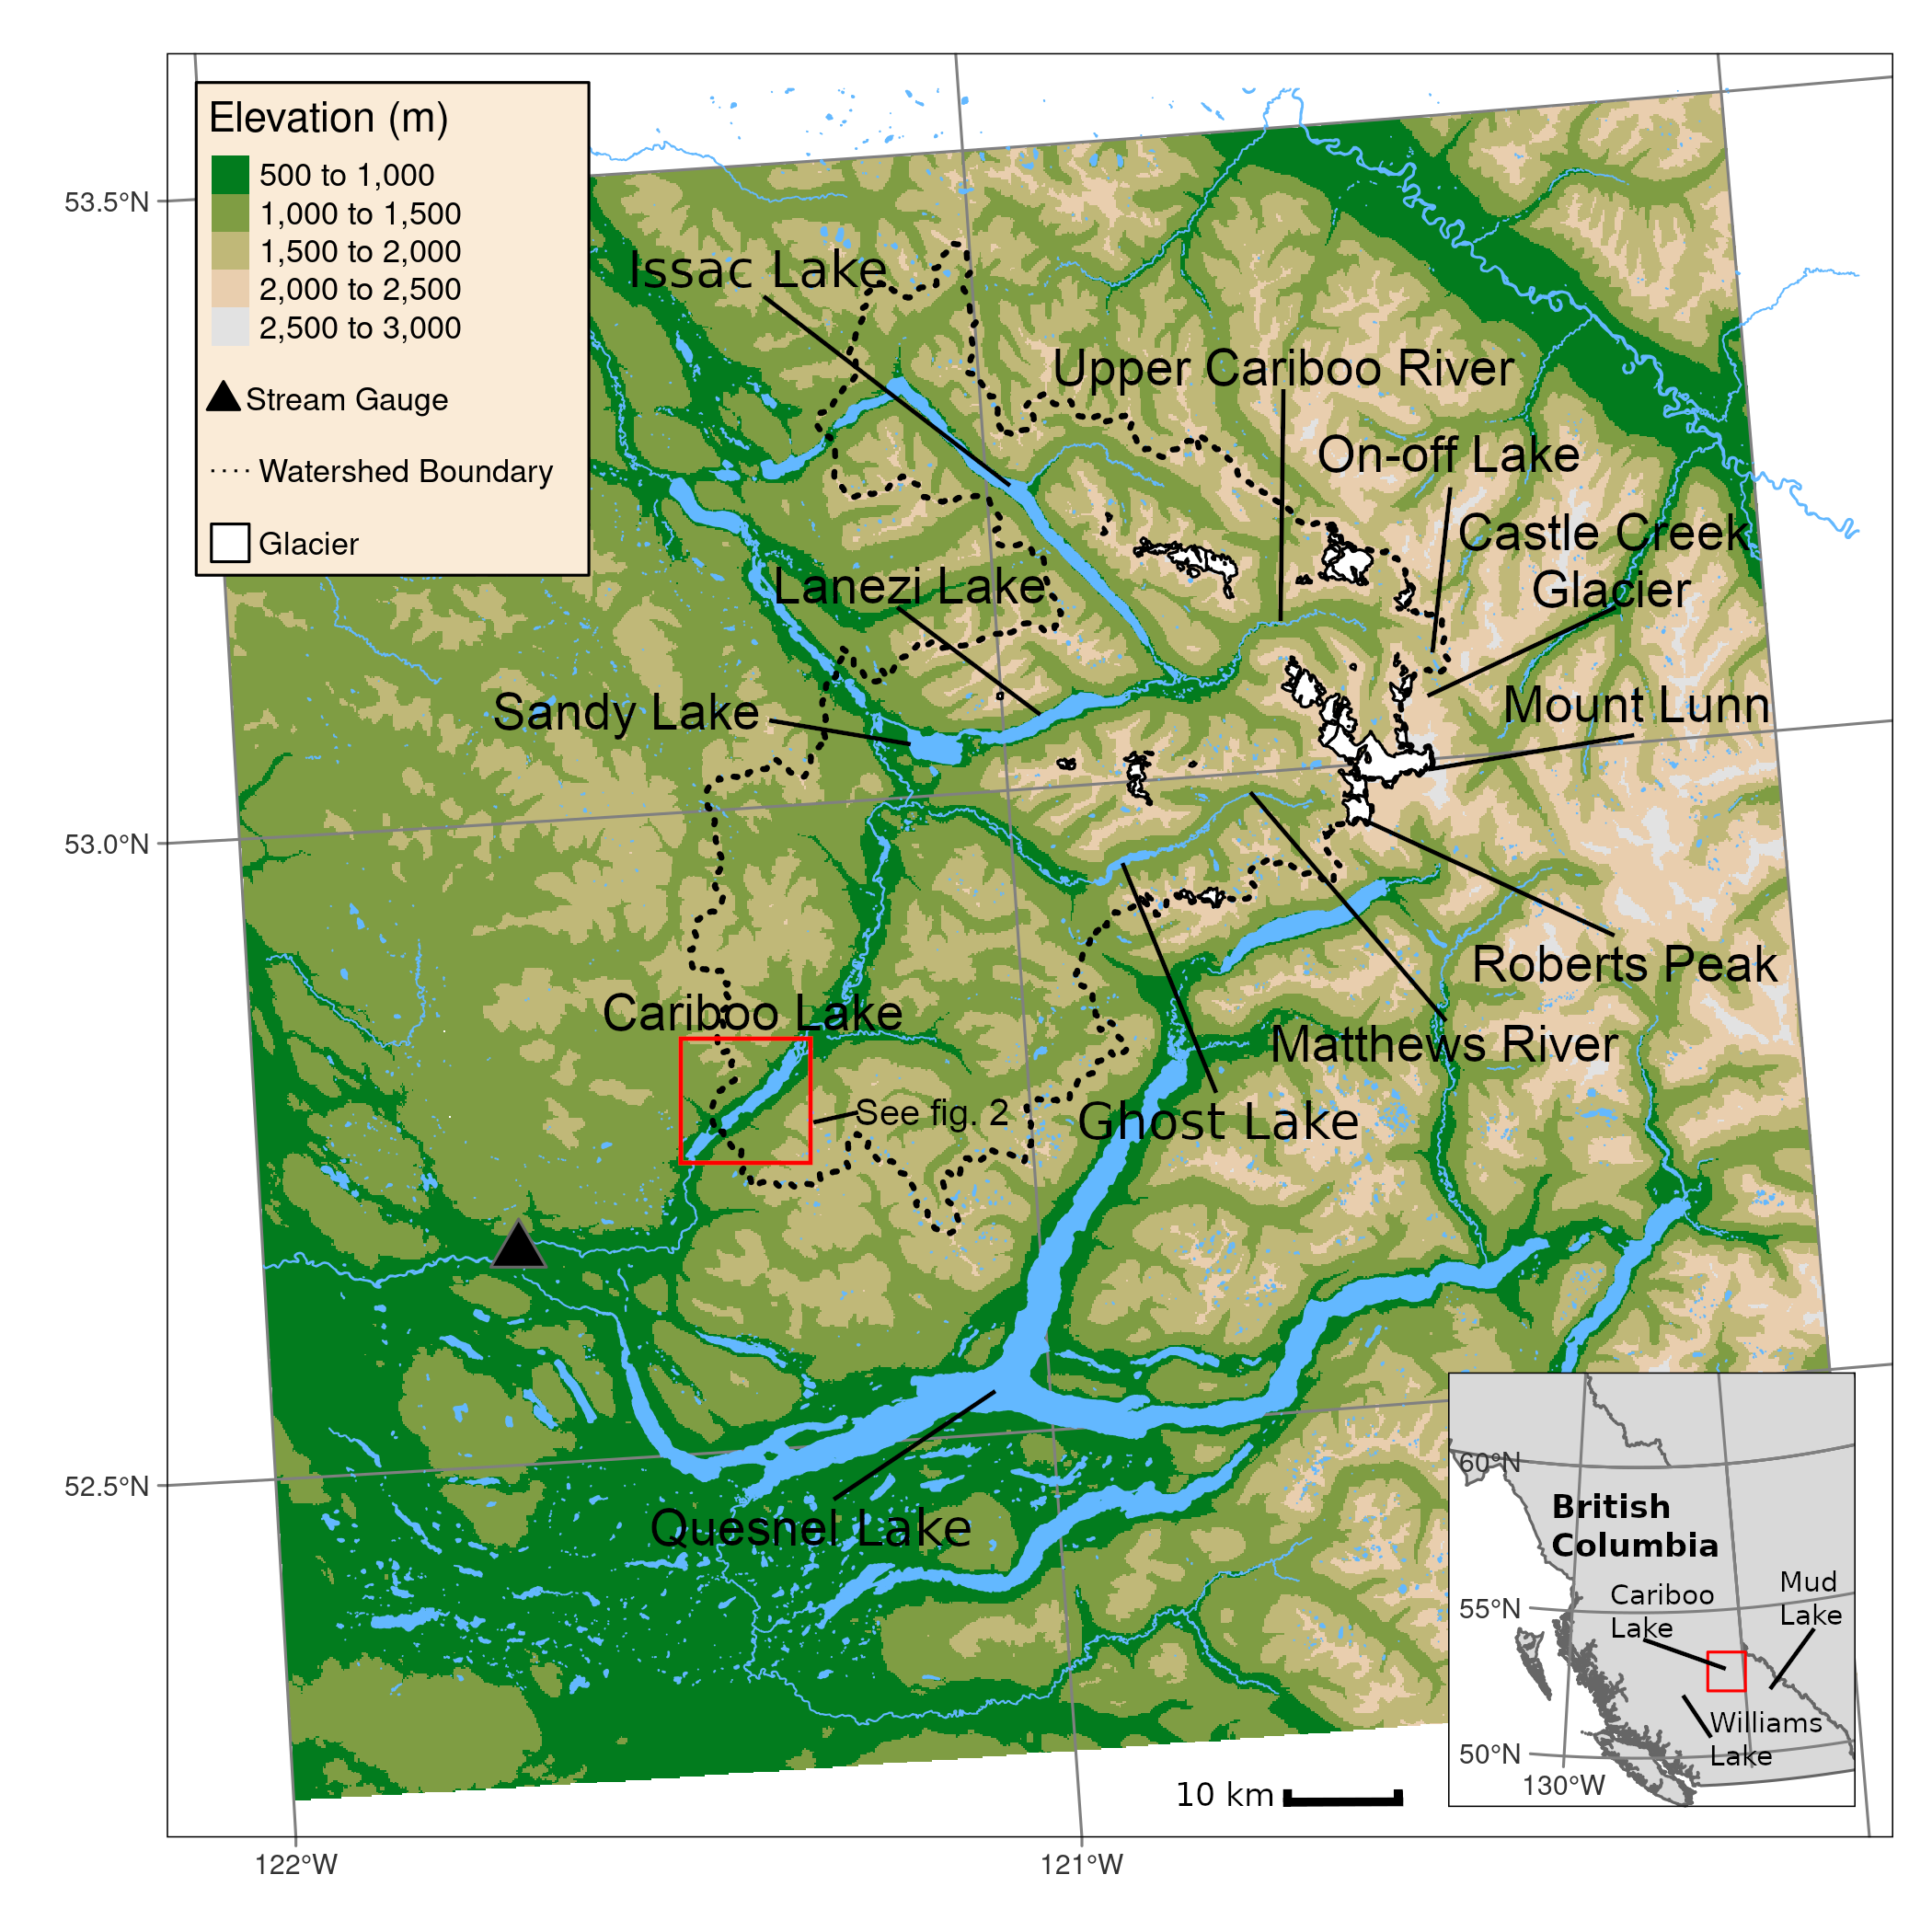
\includegraphics[width=0.95\textwidth,height=\textheight]{figs/cl_small_scale_inset_labels_gimp.png}

}

\caption{\label{fig-map-basin}\ldots{}}

\end{figure}

\begin{figure}

{\centering \includegraphics[width=1\textwidth,height=\textheight]{figs/cl_bathymetry_acoustics_coring_locations_labels.png}

}

\caption{\label{fig-map-lake}\ldots{}}

\end{figure}

\begin{figure}

{\centering 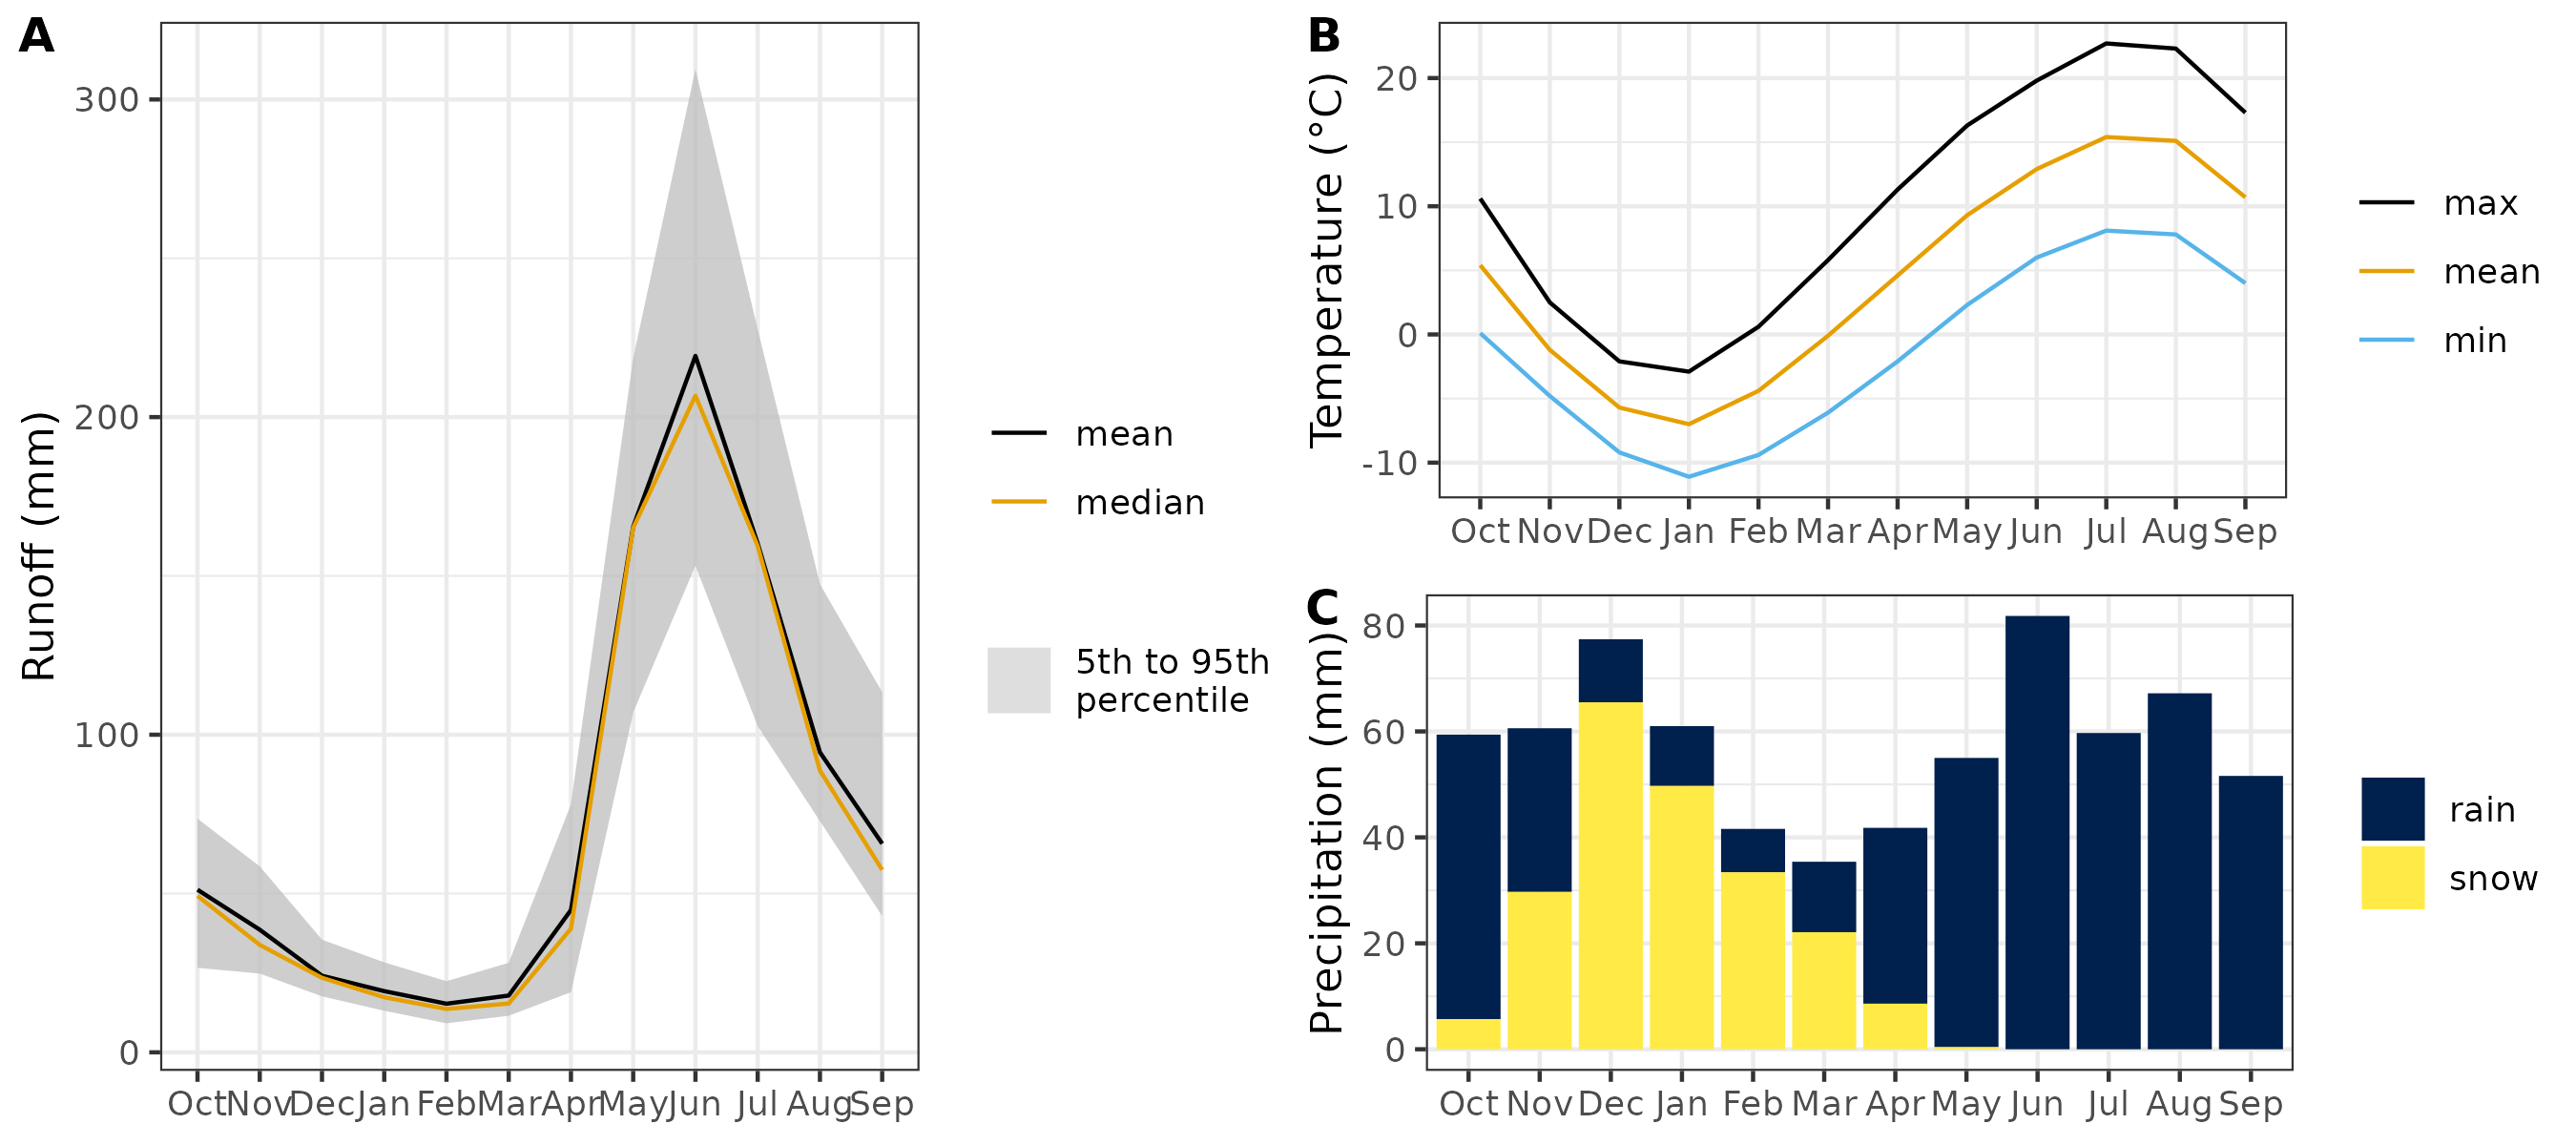
\includegraphics[width=1\textwidth,height=\textheight]{figs/cariboo_combine_climate_hydro.png}

}

\caption{\label{fig-cl-hydro}\ldots{}}

\end{figure}

\begin{figure}

{\centering \includegraphics[width=1\textwidth,height=\textheight]{../../figs/acoustics/acoustics_6_panel_cjes.png}

}

\caption{\label{fig-acoustics}\ldots{}}

\end{figure}

\begin{figure}

{\centering 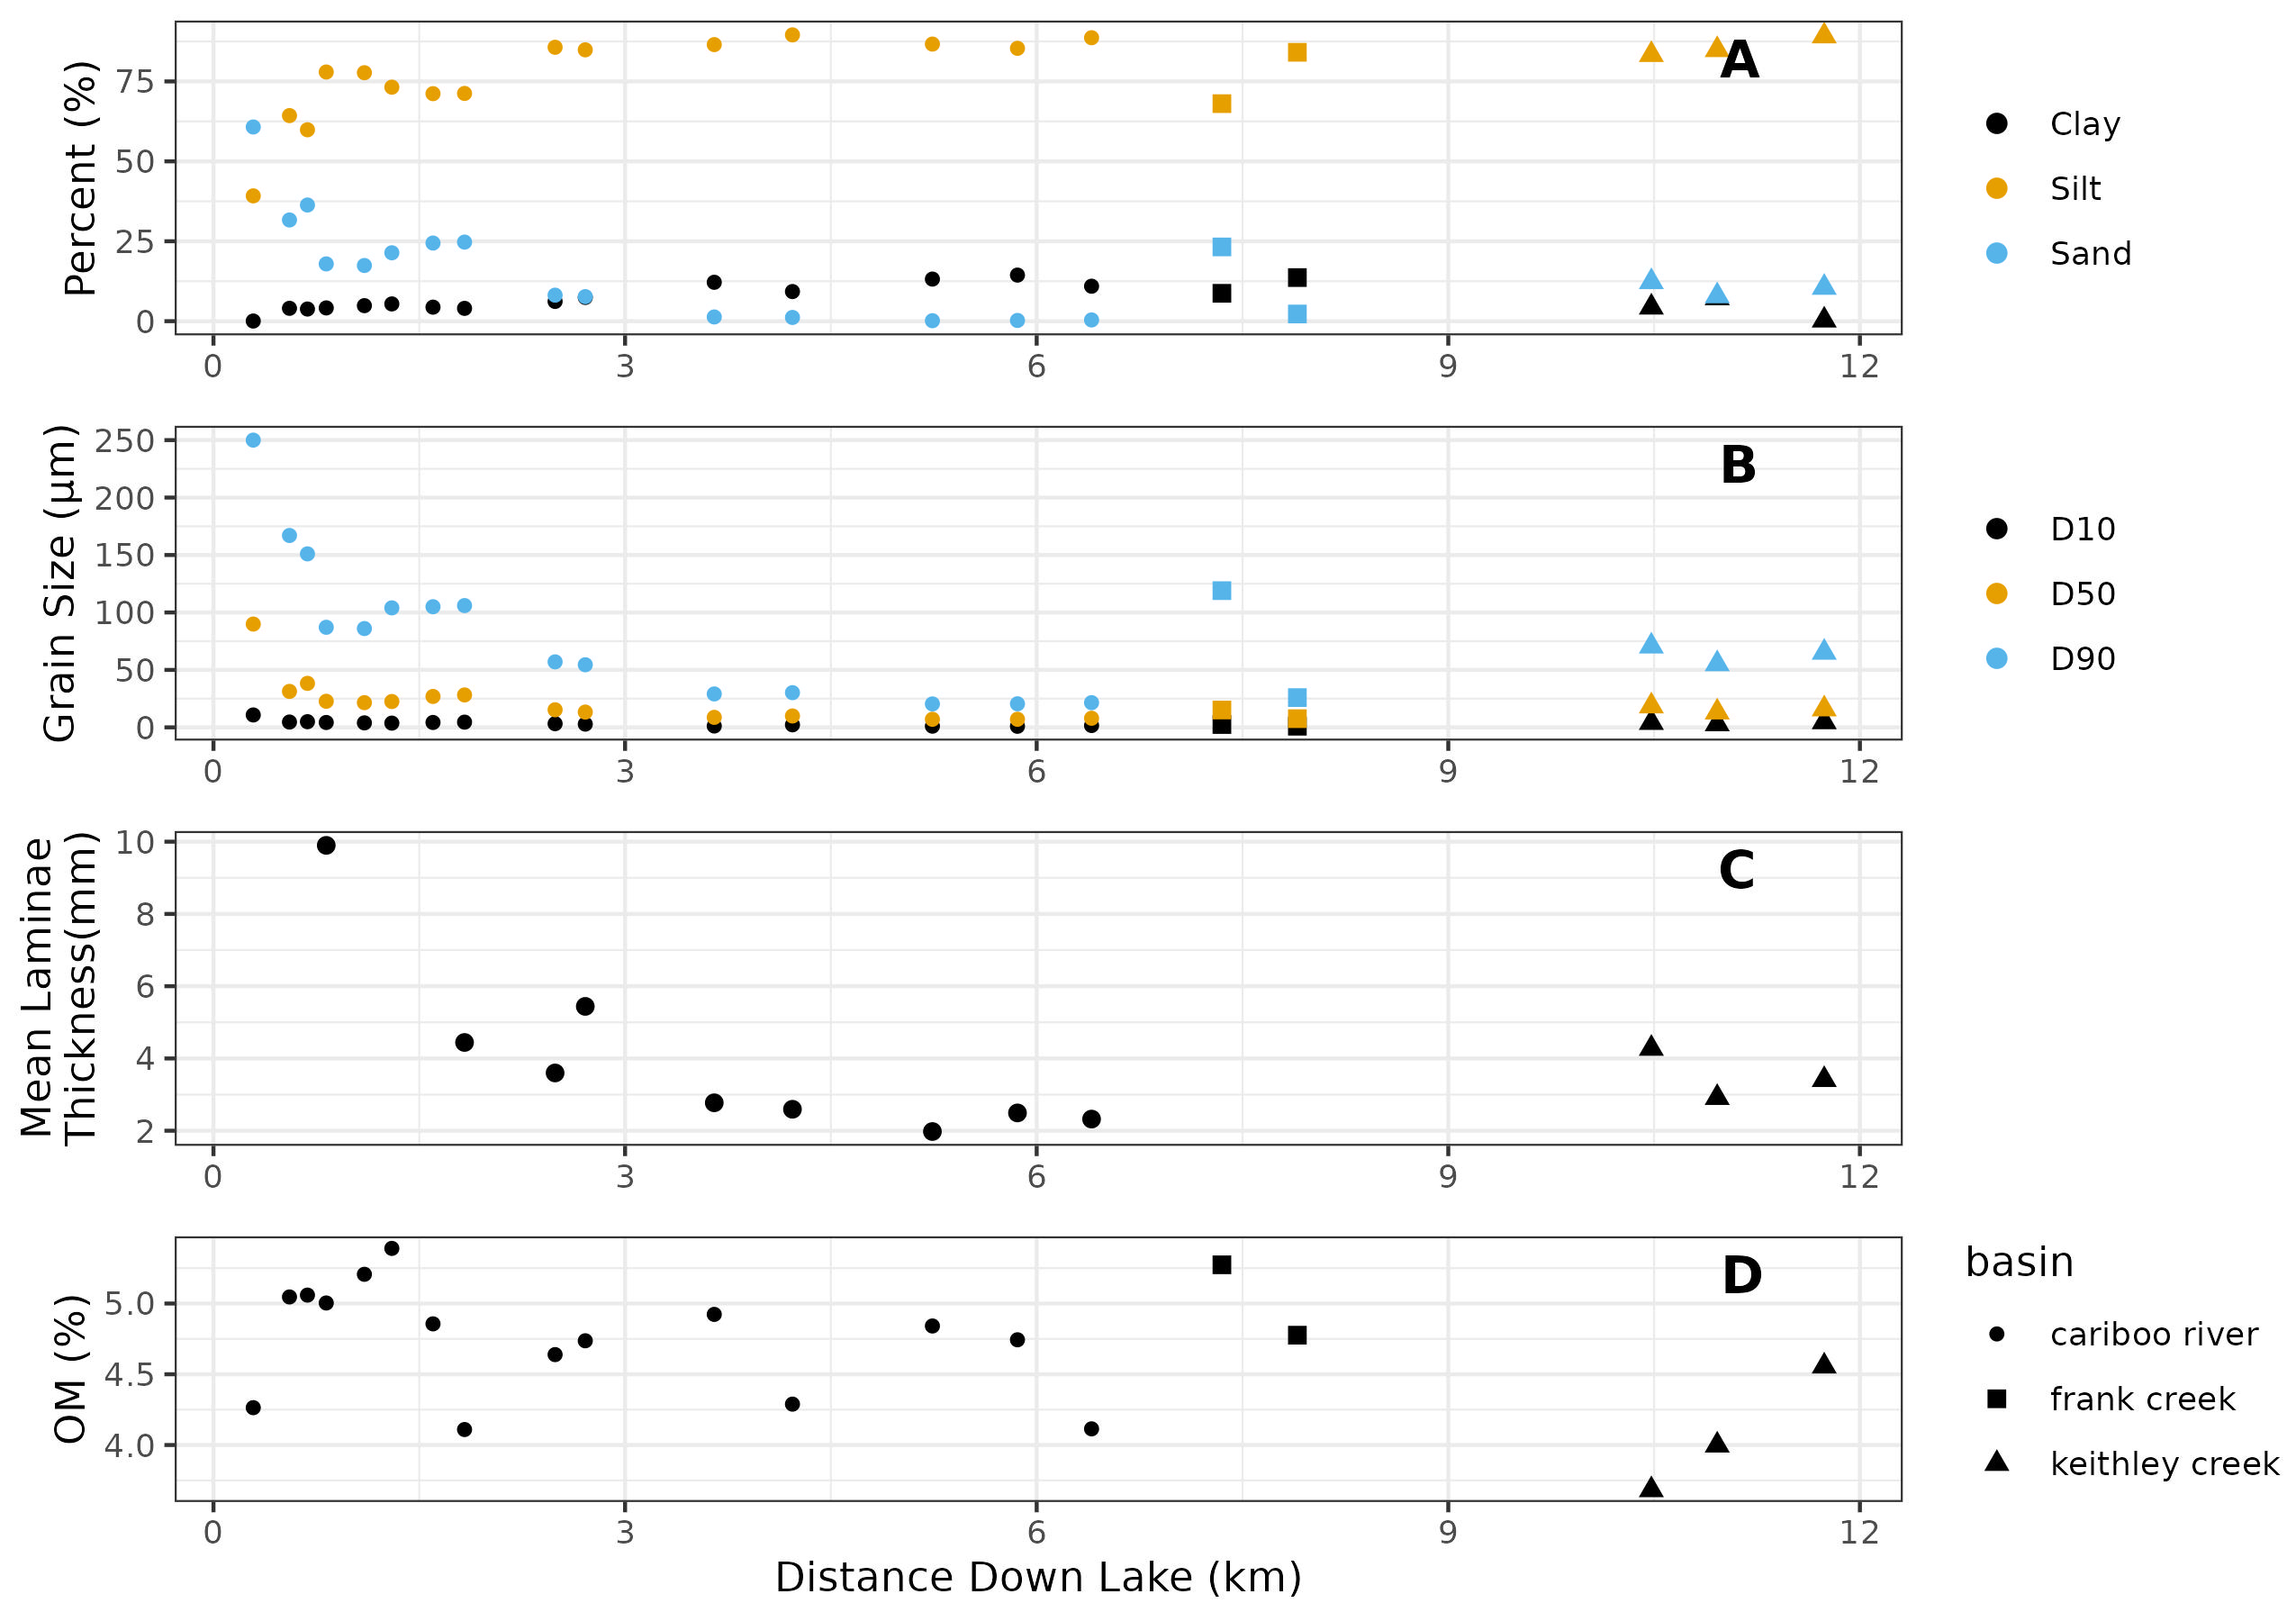
\includegraphics[width=1\textwidth,height=\textheight]{figs/ekman_seds.jpg}

}

\caption{\label{fig-ekmanSeds}\ldots{}}

\end{figure}

\begin{figure}

{\centering 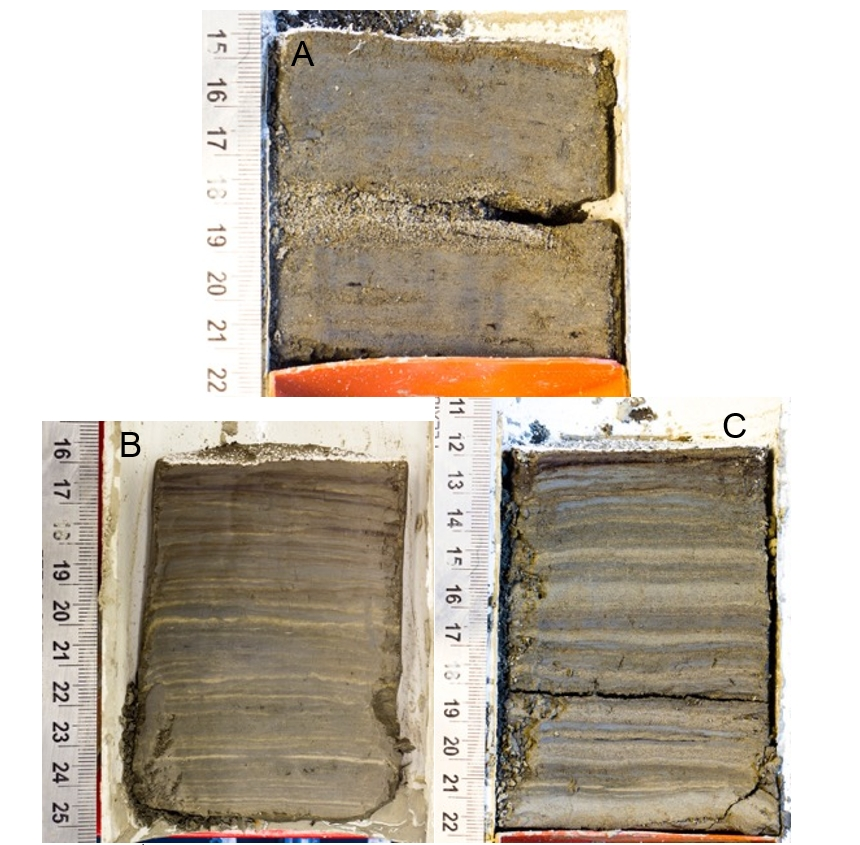
\includegraphics[width=1\textwidth,height=\textheight]{figs/ekman_example.jpg}

}

\caption{\label{fig-ekmanImgs}\ldots{}}

\end{figure}

\begin{figure}

{\centering 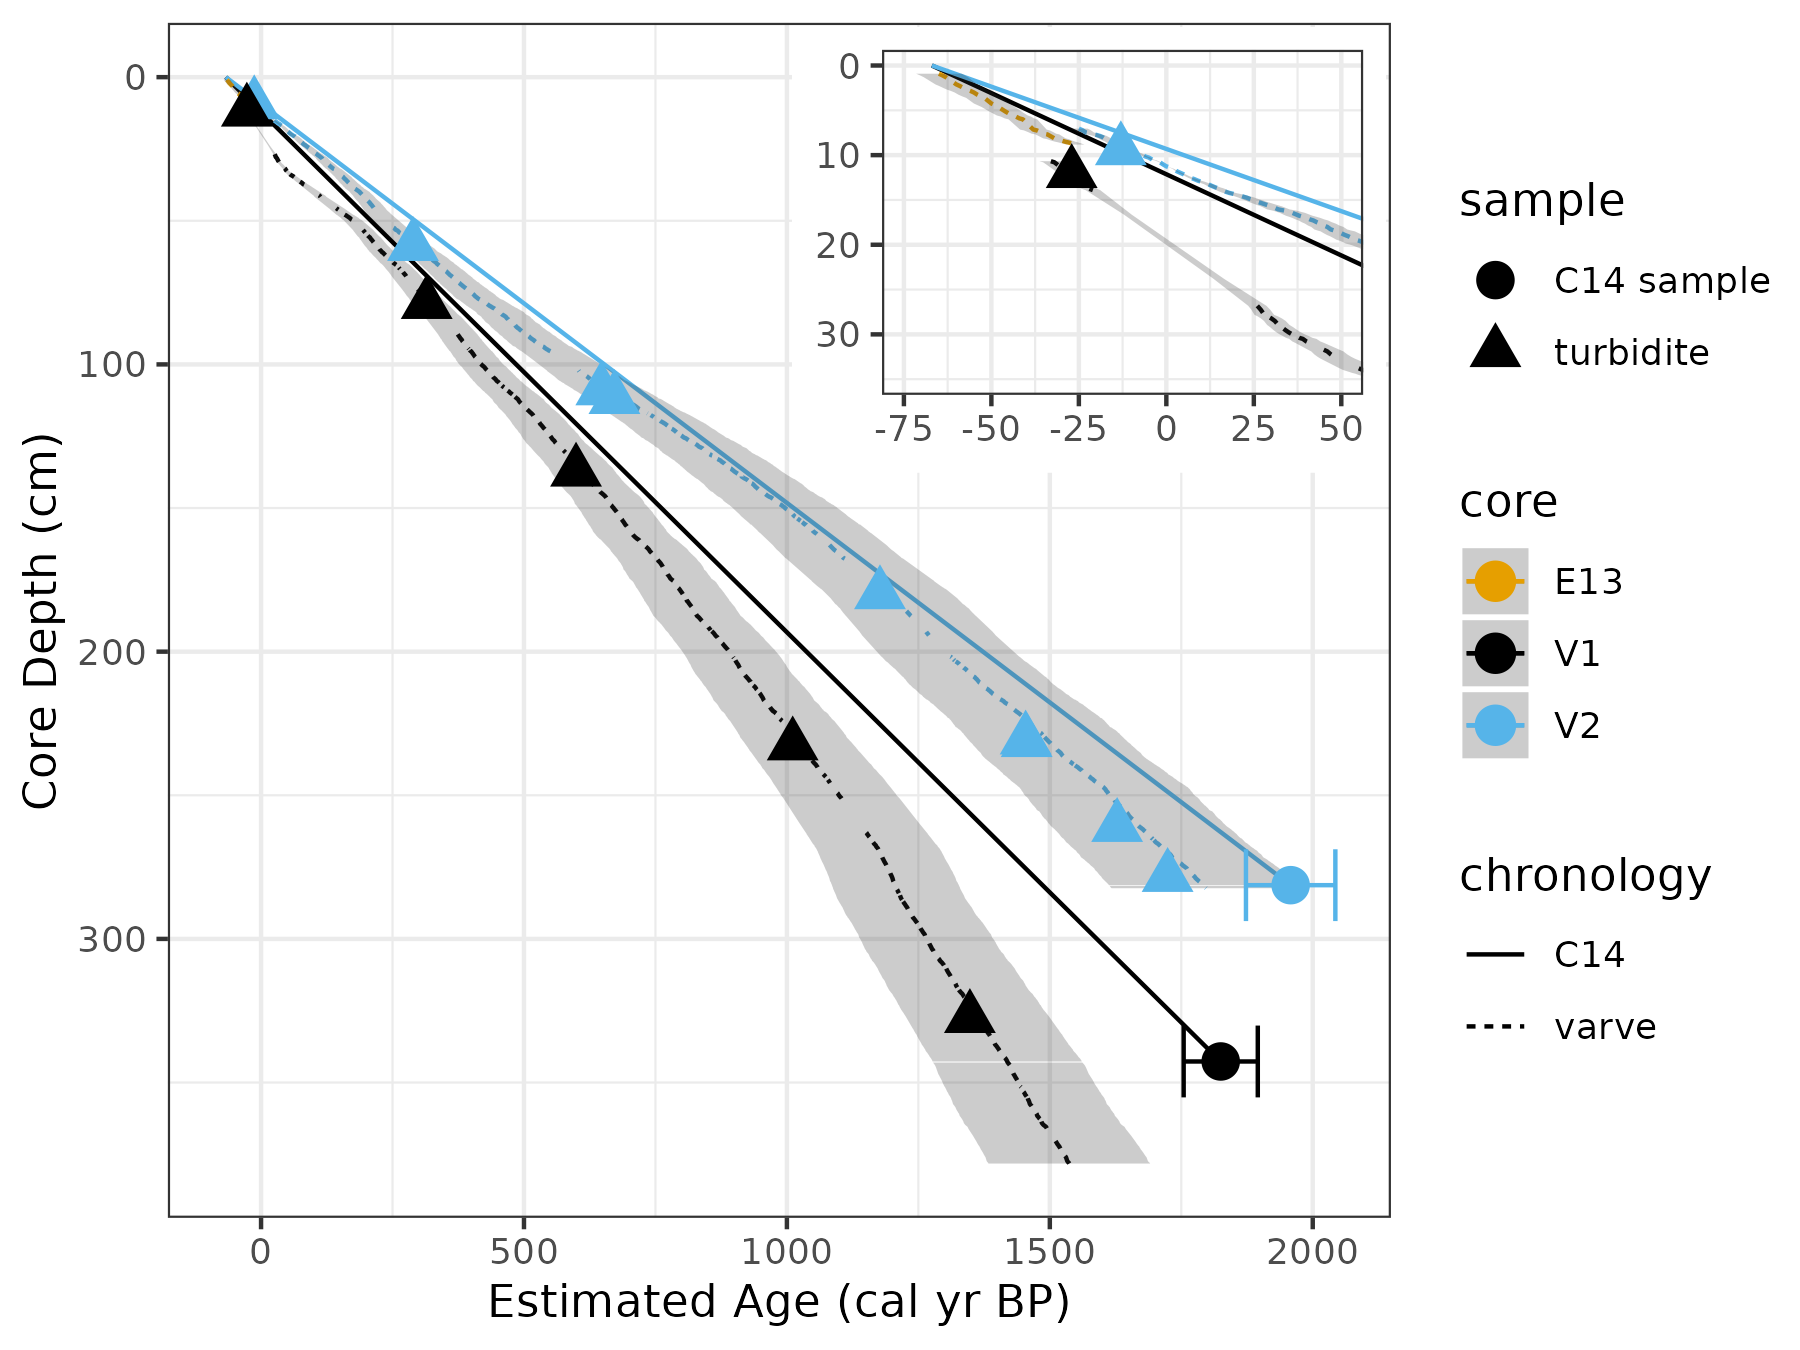
\includegraphics[width=1\textwidth,height=\textheight]{figs/longcore_cumulative_depth_vs_estimated_year_w_ams_and_varve.png}

}

\caption{\label{fig-amsRates}\ldots{}}

\end{figure}

\begin{figure}

{\centering 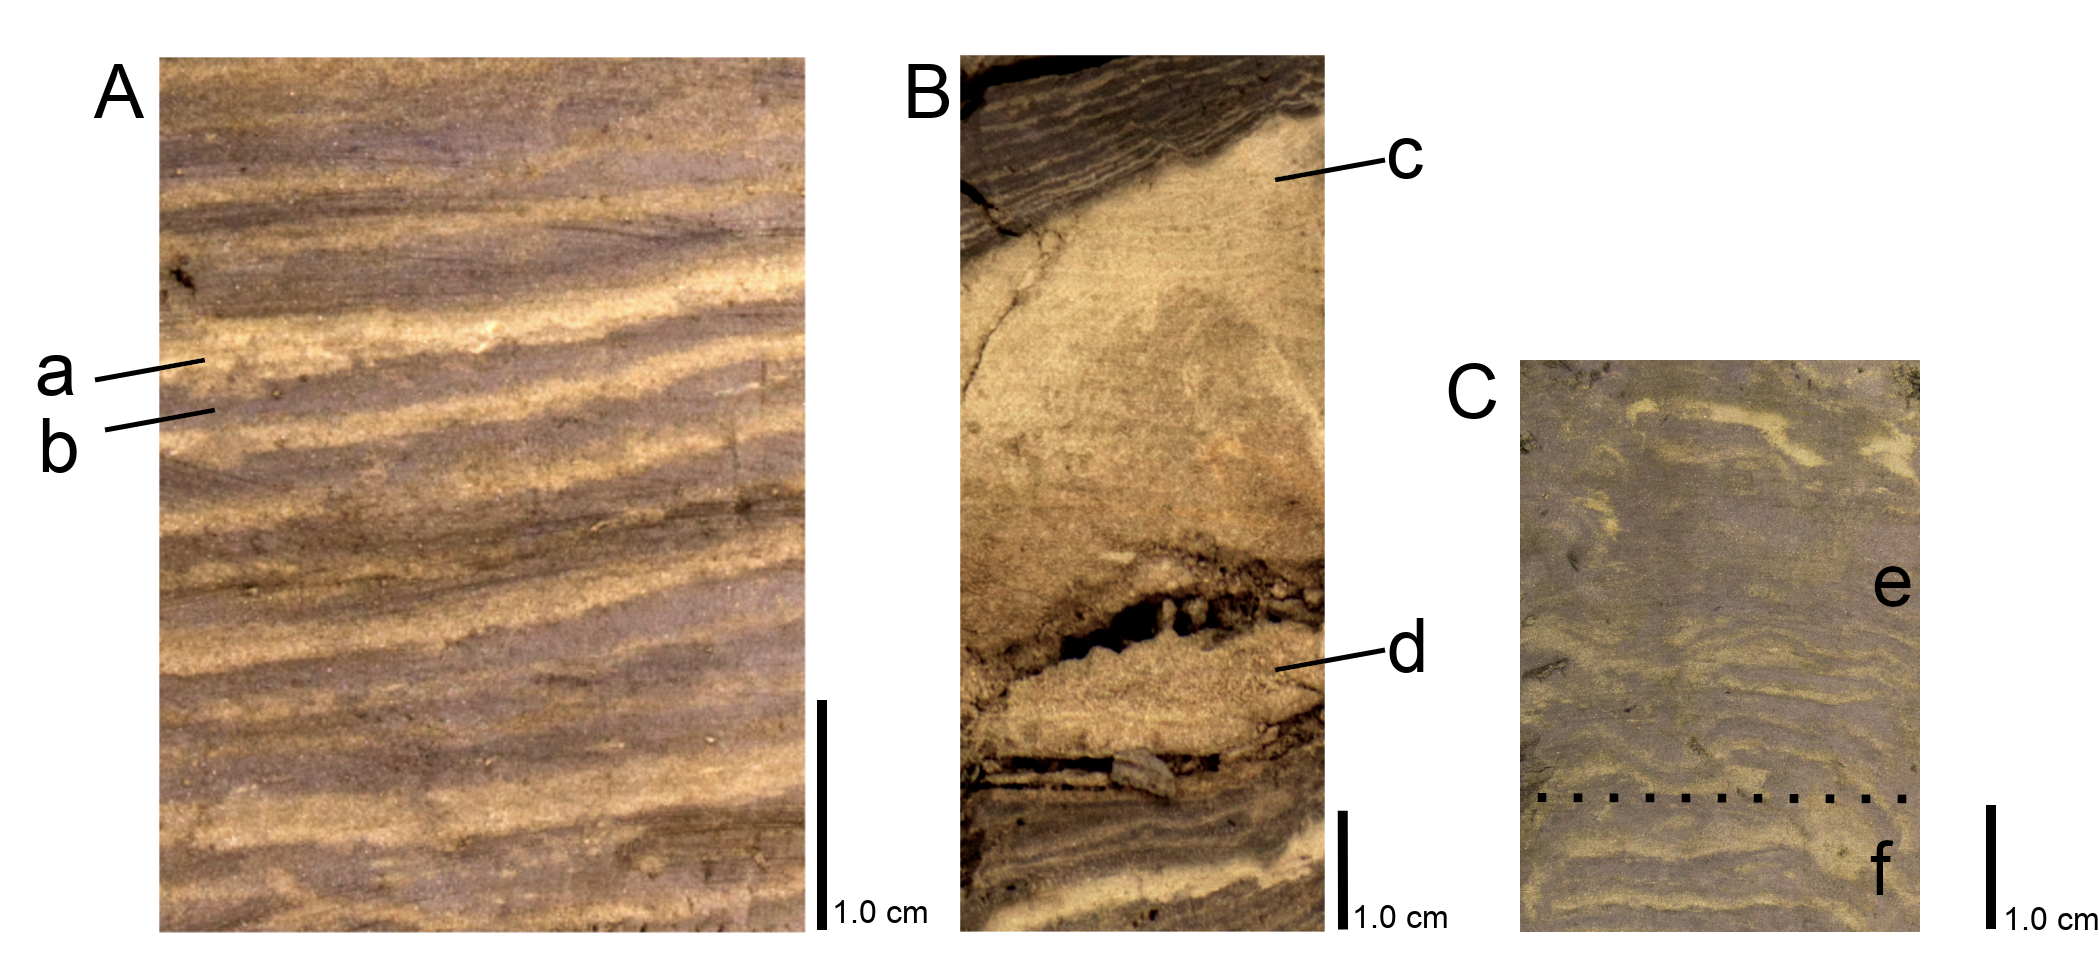
\includegraphics[width=1\textwidth,height=\textheight]{figs/good_vs_flood_vs_disturbed_varves_.png}

}

\caption{\label{fig-varve-turb}\ldots{}}

\end{figure}

\begin{figure}

{\centering 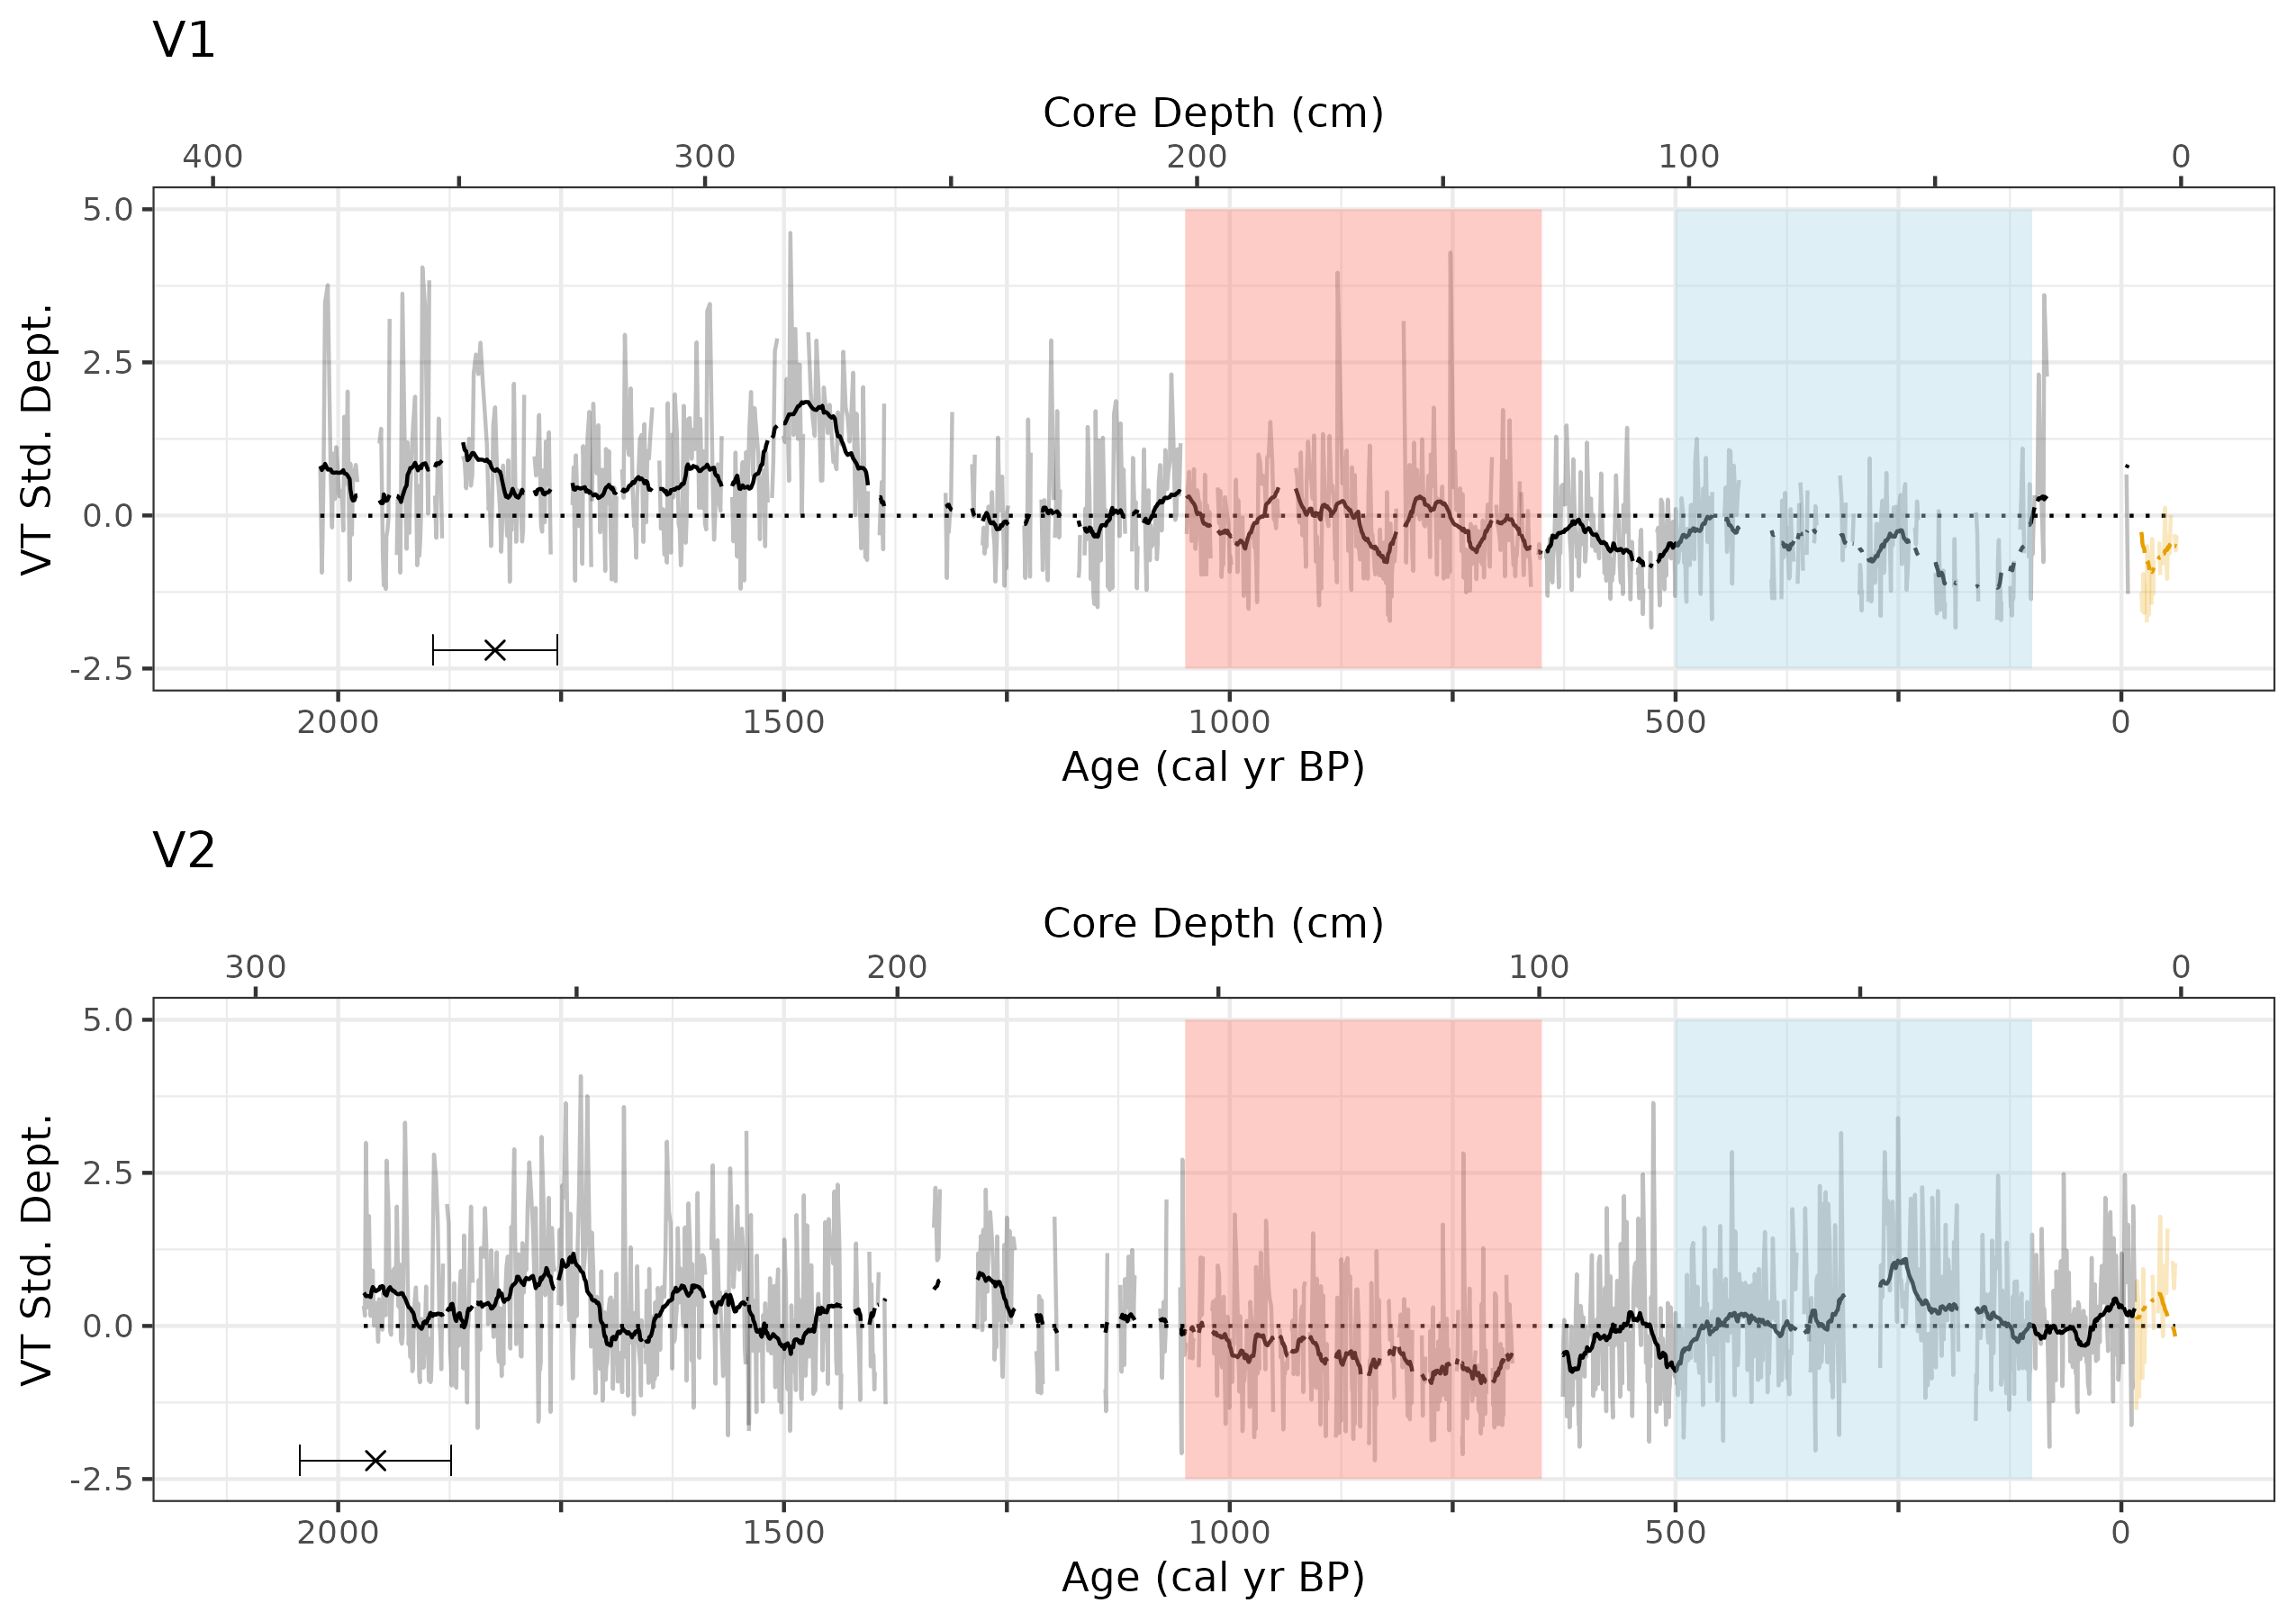
\includegraphics[width=1\textwidth,height=\textheight]{figs/V1_V2_varvethickness_vs_depth_and_C14_est_yr_ma.png}

}

\caption{\label{fig-varves-a}\ldots{}}

\end{figure}

\begin{figure}

{\centering 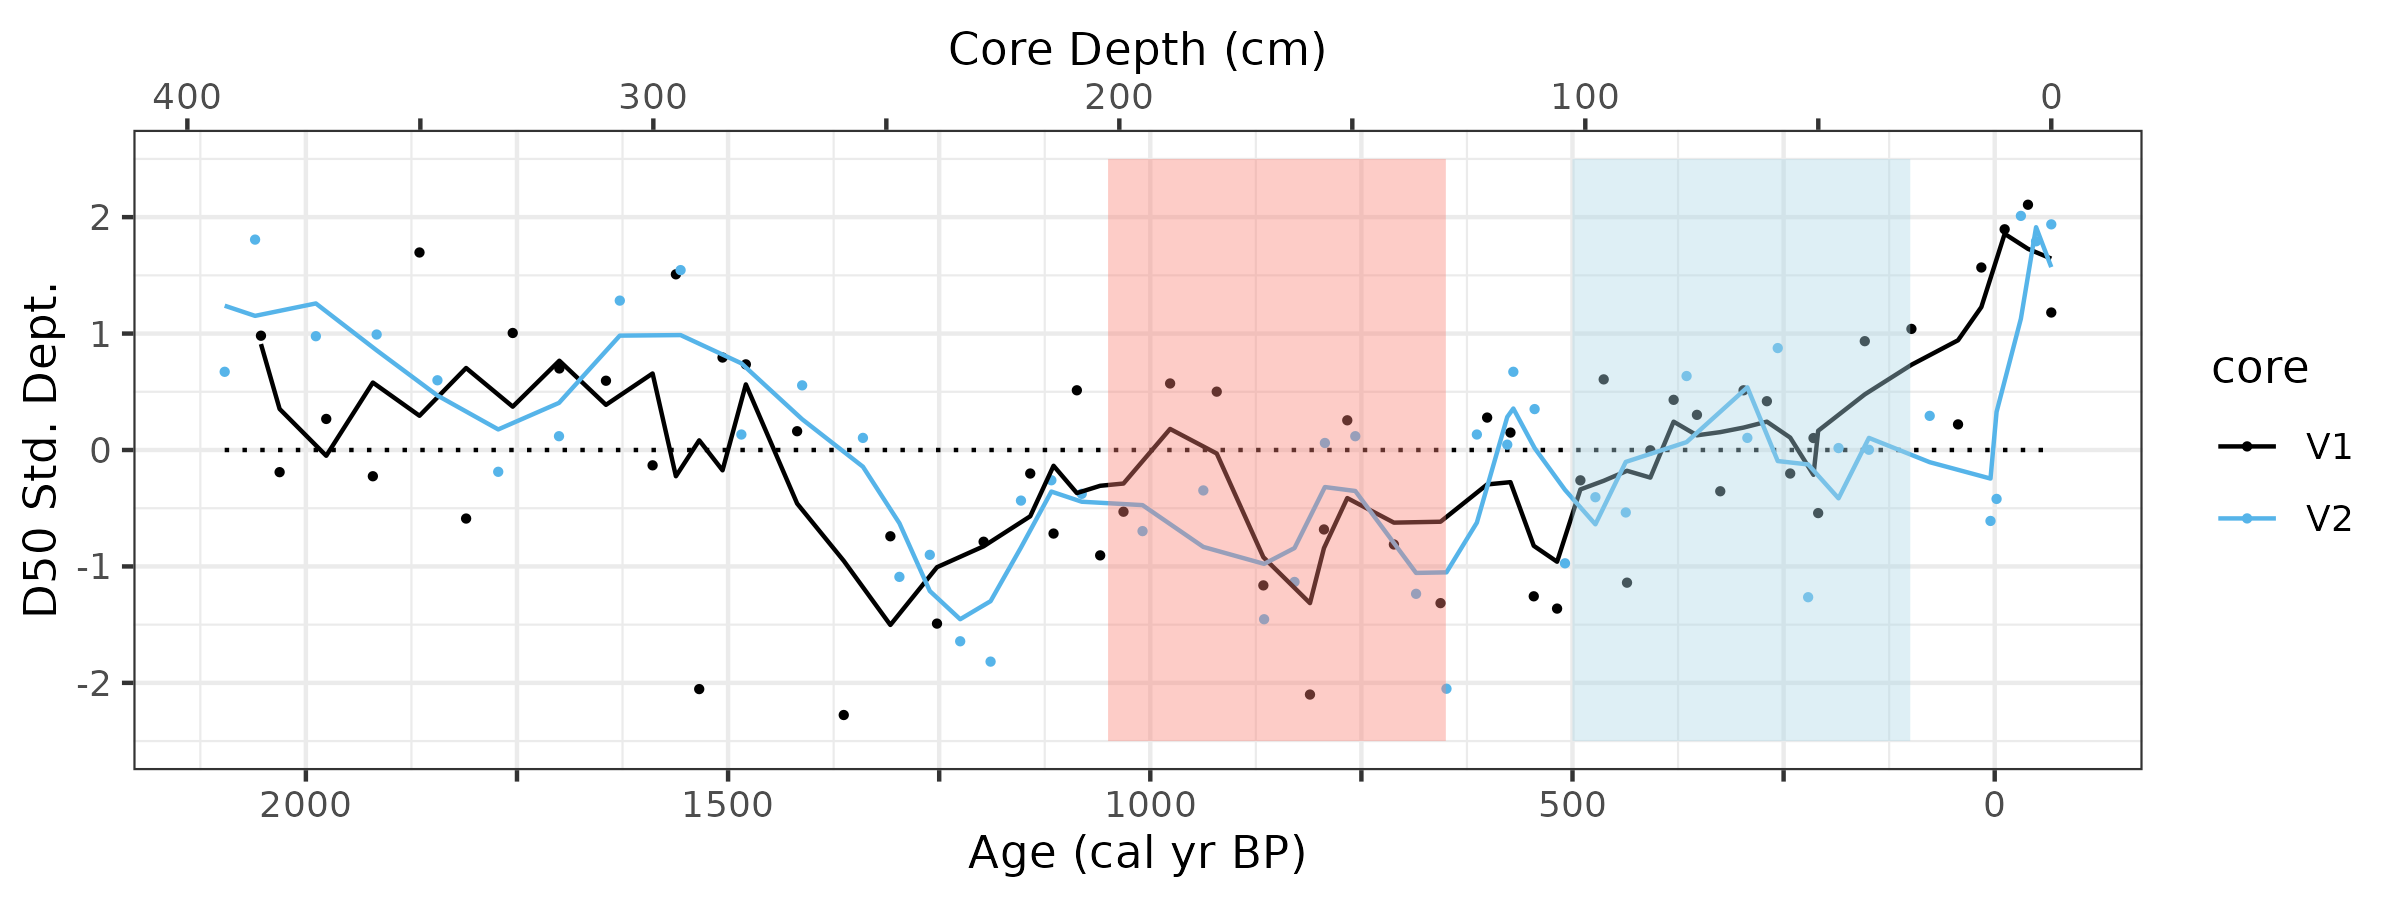
\includegraphics[width=1\textwidth,height=\textheight]{figs/V1_V2_grainsize_vs_depth_and_C14_est_yr.png}

}

\caption{\label{fig-particle}\ldots{}}

\end{figure}

\begin{figure}

{\centering 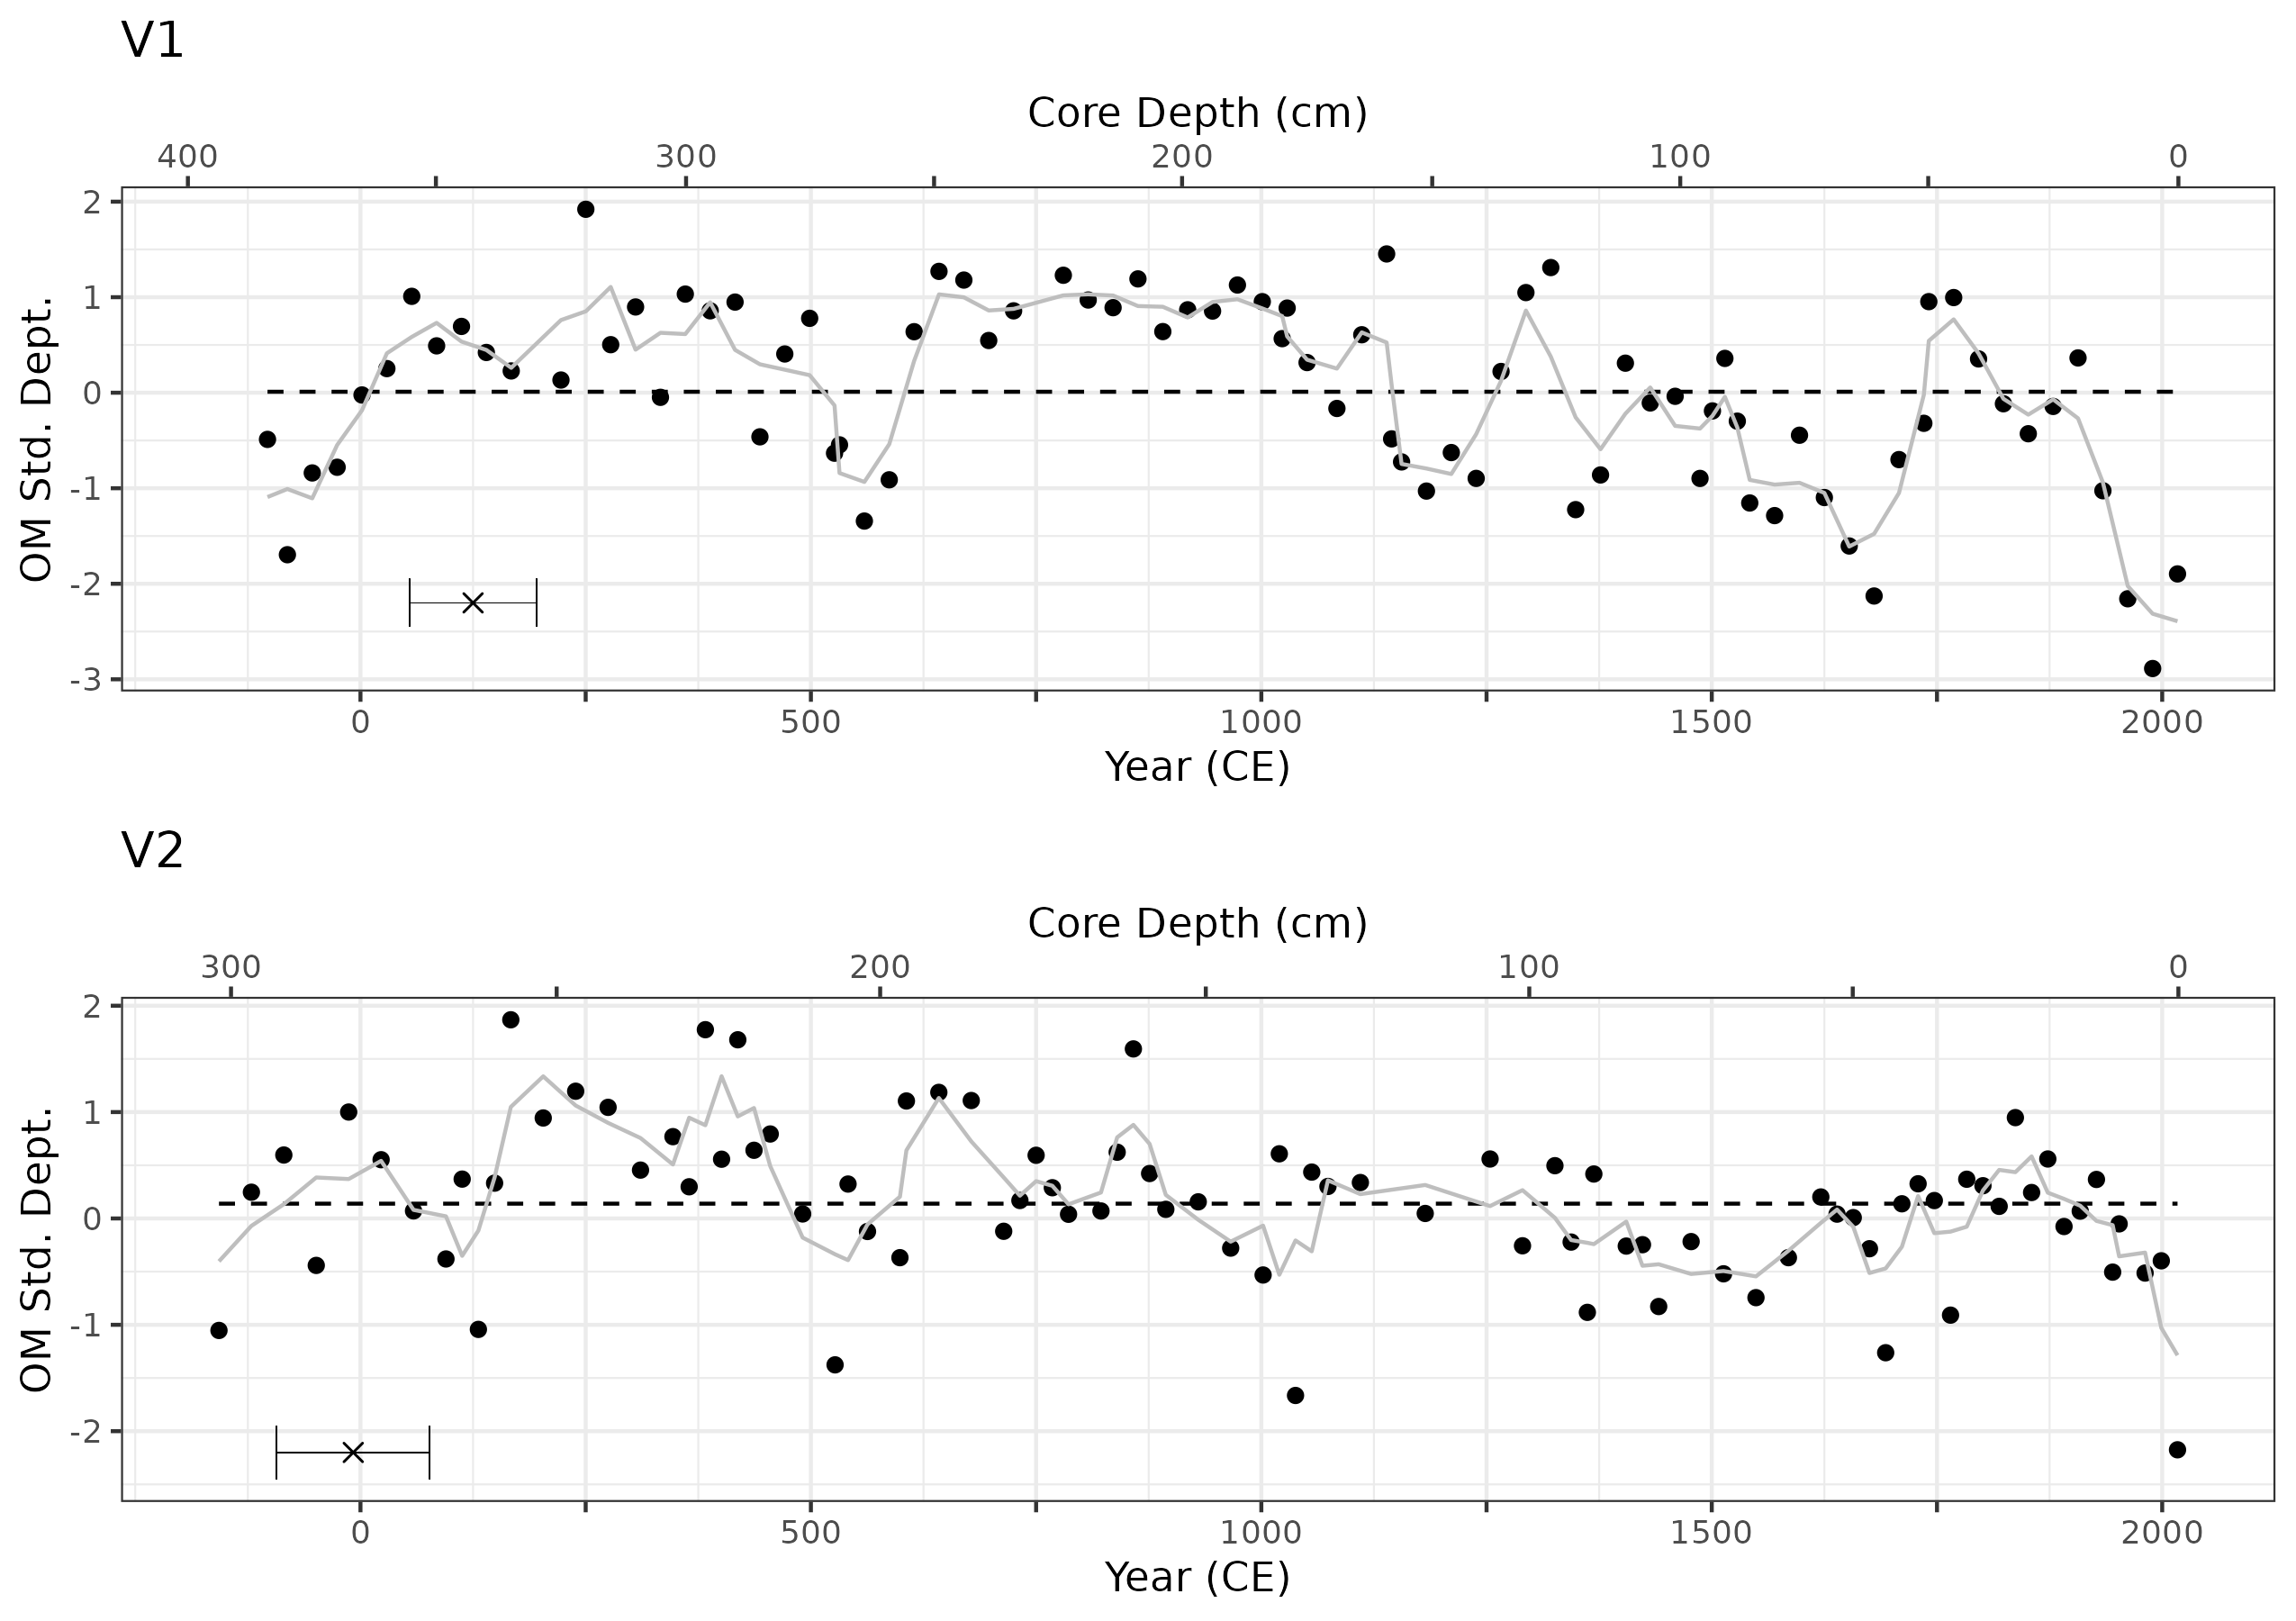
\includegraphics[width=1\textwidth,height=\textheight]{figs/V1_V2_LOI_vs_depth_and_C14_est_yr.png}

}

\caption{\label{fig-loi}\ldots{}}

\end{figure}

\begin{figure}

{\centering 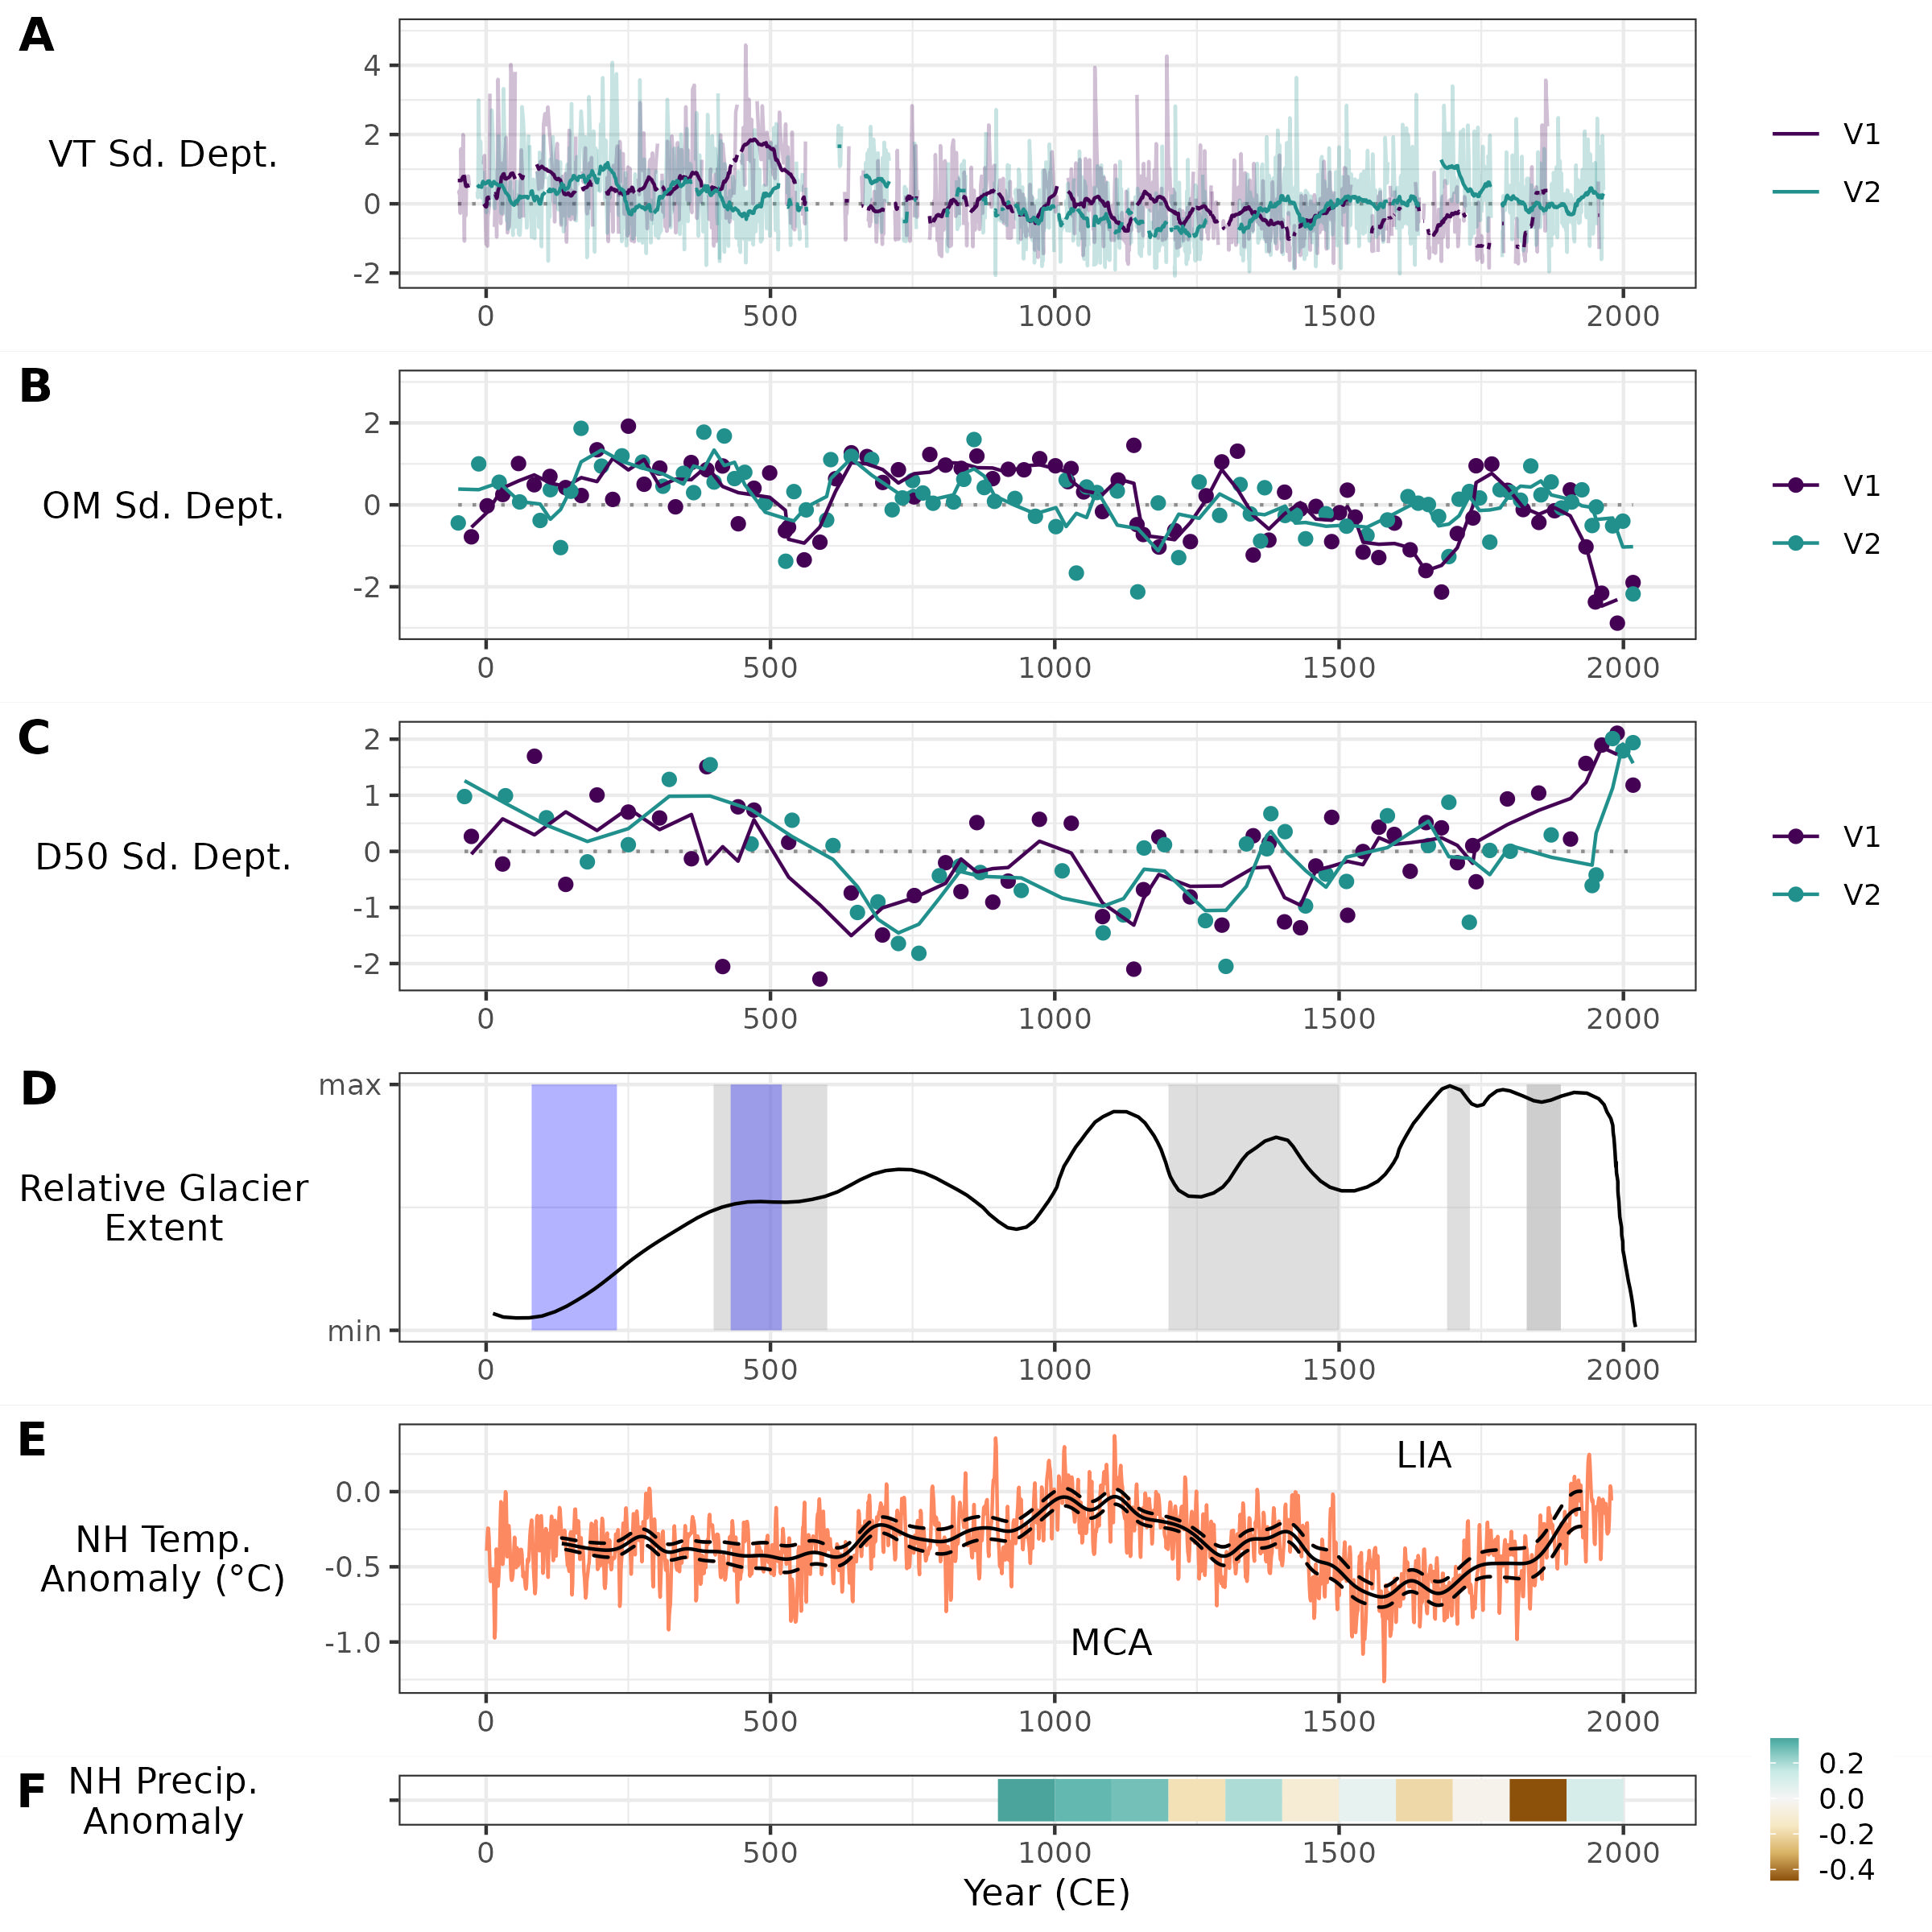
\includegraphics[width=1\textwidth,height=\textheight]{figs/all_core_stats_2k_anomalies.jpg}

}

\caption{\label{fig-proxy-comparison}\ldots{}}

\end{figure}

\pagebreak

\hypertarget{appendix}{%
\section{Appendix}\label{appendix}}

\hypertarget{tbl-ekErr}{}
\begin{longtable}[]{@{}rrr@{}}
\caption{\label{tbl-ekErr}Counting error statistics from three Ekman
short cores.}\tabularnewline
\toprule\noalign{}
Core ID & Depth (cm) & Couplet Count \\
\midrule\noalign{}
\endfirsthead
\toprule\noalign{}
Core ID & Depth (cm) & Couplet Count \\
\midrule\noalign{}
\endhead
\bottomrule\noalign{}
\endlastfoot
12 & 5 & 10 \\
13 & 5 & 12 \\
14 & 5 & 12 \\
\end{longtable}



\end{document}
